% \documentclass[output=paper,colorlinks,citecolor=brown]{langscibook}
\ChapterDOI{10.5281/zenodo.15148178}
\documentclass[output=paper,colorlinks,citecolor=brown,draft,draftmode]{langscibook}
\author{Nicholas Rolle\affiliation{Princeton University; The Leibniz-Centre General Linguistics (ZAS), Berlin}\orcid{0000-0002-1263-5930}}
\title{A tonological rarity: Tone-driven epenthesis in Ghomala'}

\abstract{This chapter focuses on a rarely mentioned tonological rarity -- tone-driven vowel epenthesis -- and argues that it is attested in the Cameroonian language Ghomala'. 
Specifically, an epenthetic vowel is inserted to avoid a rising tone on a syllable closed by an obstruent (e.g. /g\v{ɔ}p/ → [g\`ɔp\'ə] `hen'),
but  is never triggered in other tonal contexts (e.g. 
/b\^ɔp/ → [b\^ɔp] `thorax', *[b\'ɔp\`ə]).
Morpho-phonological alternations show that when this rising tone is modified and lost, the epenthetic vowel is also lost, demonstrating strict co-variation between tone and segment. 
Unlike most cases of vowel epenthesis in the literature, epenthesis cannot be attributed solely to segmental or syllabic well-formedness.
This chapter catalogues all supporting evidence for tone-driven epenthesis in Ghomala', including instrumental analysis of recordings made approximately forty years apart. 
We show that while the motivation for this process is quite common typologically (avoiding a contour tone on a sub-optimal host), the repair itself (i.e. epenthesis)  is virtually unprecedented in the literature.
    % We end by discussing two possible explanations for this rarity: 
    % the low functional load of tone, 
    % the analytic indeterminacy of epenthesis,
    % and  the potential for tone to find a pre-existing host.

\keywords{tone, contour tone, epenthesis, codas, tone-segment interaction}
}    
    % /k\'ɔp/ → [k\'ɔp] `pot', *[k\'ɔp\'ə];





\IfFileExists{../localcommands.tex}{
  \addbibresource{../localbibliography.bib}
  \usepackage{tabularx, multicol, multirow, longtable}
\usepackage{url}
\urlstyle{same}

\usepackage{orcidlink}
\definecolor{orcidlogocol}{cmyk}{0,0,0,1}
\RenewDocumentCommand{\LinkToORCIDinAffiliations}{ +m }
  {%
    \orcidlink{#1}\,%
  }
\SetupAffiliations{orcid placement=before}

\usepackage{siunitx}
\sisetup{detect-weight=true, detect-family=true, group-digits=none}

\usepackage{mathtools}
\usepackage{langsci-optional}
\usepackage{langsci-lgr}
\usepackage{langsci-gb4e}

\usepackage{stmaryrd}
\usepackage[capitalize]{cleveref}
\babelfont[macedonian]{rm}[Language=Macedonian,ItalicFont=LibertinusSerif-Italic.otf]{LibertinusSerif-Regular.otf}
\usepackage{eqparbox}
\usepackage[autostyle]{csquotes}
\usepackage[linguistics]{forest}

\usetikzlibrary{positioning, matrix}
\usepackage[glosses,inline]{leipzig}
\PassOptionsToPackage{xindy,toc,nopostdot}{glossaries}
\usepackage{glossary-inline}
\setglossarystyle{inline}
\makeglossaries

\usepackage{phonrule}
\usepackage{threeparttable}


\usepackage{textcomp,gensymb}


\usepackage[preservefont]{tipauni}

\usepackage[normalem]{ulem}

\usepackage{enumitem} %so lists aren't ugly
	
\usepackage{threeparttable}	%allows tables with tablenotes. note marks: †‡
	\makeatletter 
	\g@addto@macro\TPT@defaults{\footnotesize} 
	\makeatother

\usepackage{colortbl}
	\definecolor{Pink}{rgb}{0.96, 0.76, 0.76} 
	\definecolor{PaleBlue}{rgb}{0.67, 0.9, 0.93}
	\definecolor{carolinablue}{rgb}{0.6, 0.73, 0.89}
	\definecolor{goldenyellow}{rgb}{1.0, 0.87, 0.0}
	\definecolor{Orange}{rgb}{1.0, 0.66, 0.07}
	\definecolor{puce}{rgb}{0.8, 0.53, 0.6}
	\definecolor{turquoisegreen}{rgb}{0.63, 0.84, 0.71}


% add all extra packages you need to load to this file
\usepackage{langsci-textipa}
\usepackage{vowel}
\usepackage{textgreek}

% \usepackage{langsci-branding}
% \usepackage{subcaption}
\usepackage{subfigure}

\usepackage{tabto}


\usetikzlibrary{tikzmark}
\usepackage{pgfplots}


\newfontfamily\tibetan{NotoSerifTibetan-Regular.ttf}
\usepackage{langsci-branding}
\usepackage{hyphenat}

\usepackage{accents}

  \renewcommand{\lsChapterFooterSize}{\footnotesize}

\makeatletter
\let\thetitle\@title
\let\theauthor\@author
\makeatother

\newcommand{\togglepaper}[1][0]{
   \bibliography{../localbibliography}
   \papernote{\scriptsize\normalfont
     \theauthor.
     \titleTemp.
     To appear in:
     Natalia Kuznetsova, Cormac Anderson \& Shelece Easterday (ed.).
     Rarities in phonetics and phonology.tex.
     Berlin: Language Science Press. [preliminary page numbering]
   }
   \pagenumbering{roman}
   \setcounter{chapter}{#1}
   \addtocounter{chapter}{-1}
}

\newbool{bookcompile}
\booltrue{bookcompile}
\newcommand{\bookorchapter}[2]{\ifbool{bookcompile}{#1}{#2}}

\newcommand{\textarab}[1]{\RL{\arabicfont #1}}

\newcommand\mb[1]{\eqparbox[t]{examples}{#1}\hspace{1em}}
\newcommand\mbi[1]{\mb{#1}}
\newcommand{\twe}[3]{\mbi{#1}\eqparbox[t]{orths}{\emph{#2}}\hspace{1em}`#3'\hspace{1em}} % three-way example
\providecommand\glottocode[1]{[\href{https://glottolog.org/resource/languoid/id/#1}{#1}]}
\newcommand{\phonreal}[1]{\ensuremath{\llbracket}#1\ensuremath{\rrbracket}}

\DeclareRobustCommand\dash{\unskip\nobreak\thinspace\textendash\allowbreak\thinspace\ignorespaces}

\forestset{minus/.style={edge label={node[midway, left] {\ensuremath{-}\hspace*{2mm}}}},
plus/.style={edge label={node[midway, right] {\hspace*{2mm}\ensuremath{+}}}}}
\providecommand\ipa[1]{#1}


\newcommand{\tone}[1]{\textsuperscript{#1}}

\newcommand{\orthog}[1]{\textit{#1}}
\newcommand{\gloss}[1]{`#1'}

\newcommand{\glottolog}[1]{\texttt{\href{https://glottolog.org/resource/languoid/id/#1}{#1}}}

\newcolumntype{O}{>{\itshape }l<{}}
\newcolumntype{G}{>{`}l<{'}}

\newcounter{tabsubcounter}
\newcommand{\tablecounter}{\setcounter{tabsubcounter}{0}}
\newcommand{\TC}{\stepcounter{tabsubcounter}\alph{tabsubcounter}.}

\usetikzlibrary{chains,positioning,calc,decorations.markings}
\tikzset{
	seg/.style={text height=0.6em, text depth=0.3em},
	moraic-structure/.style={xscale=0.6,yscale=1.1, text height=0.65em,text depth=0.25em},
 }

%05_Culhane_Edwards
%%%%%%%%%%%%%%%%%%%%%%%%%%%%%%%%
%%	Symbols and Characters  	%%
%%%%%%%%%%%%%%%%%%%%%%%%%%%%%%%% αβσµ

\newcommand{\tl}{\char`~}						%middle tilde ~
\renewcommand{\Q}{\textquotesingle}		%straight apostrophe444
\newcommand{\ra}{→} 								%right arrow ->
\newcommand{\0}{∅} 									%zero symbol
\newcommand{\gap}{\textunderscore} 	%underscore
%\renewcommand{\j}{ʤ}								%dezh digraph
\newcommand{\syll}{σ}								%lowercase sigma medial form
\newcommand{\wrd}{ω}								%lowercase omega
\newcommand{\ft}{φ}									%lowercase phi
\newcommand{\gw}{gʷ}								%g with superscript w
\newcommand{\B}{β}									%voiced bilabial fricative
\newcommand{\hp}{\hphantom}					%space equal to width of argument
\newcommand{\it}{\textit}	%italics

%%%%%%%%%%%%%%%%%%%%%%%%%%%%%%%%
%%	Font Styles & Formatting	%%
%%%%%%%%%%%%%%%%%%%%%%%%%%%%%%%%

\definecolor{DarkBlue}{RGB}{0,0,130}										%dark blue colour
% \newcommand{\ve}[1]{\textcolor{DarkBlue}{\textit{#1}}}	%vernacular text
\newcommand{\ve}[1]{{\textit{#1}}}	%vernacular text
\definecolor{DarkRed}{RGB}{150,0,0}											%dark red colour
% \newcommand{\tbr}[1]{\textcolor{DarkRed}{\textbf{#1}}}	%Bold red text
\newcommand{\tbr}[1]{{\textbf{#1}}}	%Bold red text
%\renewcommand{\it}{\textit}																%italics
\newcommand{\tsc}{\textsc}															%small caps
\newcommand{\sub}{\textsubscript}												%subscript
\newcommand{\su}{\textsuperscript}											%superscript

%%%%%%%%%%%%%%%%%%%%%%%%%%%%%%%%%%%%%%%%%%%%%%%%%%%%
%% Tables %% Tables %% Tables %% Tables %% Tables %%
%%%%%%%%%%%%%%%%%%%%%%%%%%%%%%%%%%%%%%%%%%%%%%%%%%%%

% \newcommand{\mc}{\multicolumn}									%multicolumn
% \newcommand{\st}[1]{\setlength{\tabcolsep}{#1}}	%reduce column width in tables
%
%%%%%%%%%%%%%%%%%%%%%%%%%%%%%%%%
%%    Cross   References      %%
%%%%%%%%%%%%%%%%%%%%%%%%%%%%%%%%

% \def\Plus{\texttt{+}}
% \def\Minus{\texttt{-}}
% \newcommand{\GS}{ʔ}
% \def\SH{ʃ}
% \newcommand{\TSH}{ʧ}
% \def\ZH{ʒ}
% \def\DZH{ʤ}
% \def\:{ː}
% \def\UP{\textsuperscript}
% \def\rs{ʂ}
% \newcommand{\rn}{ɳ}
% \def\rt{ʈ}
% \def\tllr{ɺ}
% \newcommand{\Bb}{β}
% \def\Eps{ɛ}
% \def\Oo{ɔ}
% \def\Gm{ɣ}
% \def\NG{ŋ}
% \def\barU{ʉ}
\newcommand{\CM}{\ding{51}}
\newcommand{\XM}{\ding{53}}
% \newcommand{\tap}{ɾ}
% \def\darkL{ɫ}
% \def\schwa{ə}
%
% \def\BUL{\textbullet}


%%%%%%%%%%%%%%
%					%
%	Secondaries		%
%					%
%%%%%%%%%%%%%%
%	Post
\newcommand{\Post}[2]{#1\textsuperscript{#2}}
%	Pre
\newcommand{\Pre} [2] {\textsuperscript{#1}#2}
%	Undertilde
\newcommand{\utilde}[1]{\ensuremath{\smash{\underset{\mathclap{\sim}}{\text{#1}}}}}
%	Devoiced
% \newcommand{\VCLS}[1]{\textsubring{#1}}
%%%%%%%%%%%
%				%
%	Definitions		%
%	Markup		%
%				%
%%%%%%%%%%%
% \def\->{$\rightarrow$}
% \def\__{\underline{\hspace{1em}}}
\def\NoPoss{\cellcolor{gray!30}}

\newcommand{\VOICELESS}{\textsc{voiceless}}
\newcommand{\VOICED}{\textsc{voiced}}
\newcommand{\tablenote}[2][1]{\parbox{#1\textwidth}{\footnotesize\raggedright #2}}

\newcommand{\appref}[1]{Appendix~\ref{#1}}
\renewcommand{\sectref}[1]{Section~\ref{#1}}


\newcommand{\dobuibox}[5]{#1\\[-1.1em]
\hspace*{-.8cm}
 \begin{tabularx}{.9\textwidth}{@{}lQQ@{}}
       &  {oral} &  {nasal} \\
       \midrule
     {controlled} &\parbox[t]{4cm}{\raggedright  #2} & \parbox[t]{4cm}{\raggedright #3} \\
     \tablevspace
     {ballistic} &\parbox[t]{4cm}{\raggedright  #4} & \parbox[t]{4cm}{\raggedright  #5} \\
 \end{tabularx}
}

\newfontfamily\VdottildeFont{LibertinusVdottilde.otf}

\newcommand{\Vdottilde}{{\VdottildeFont V̰̣}}

% \renewcommand{\keywords}[1]{\textbf{#1}}

  %% hyphenation points for line breaks
%% Normally, automatic hyphenation in LaTeX is very good
%% If a word is mis-hyphenated, add it to this file
%%
%% add information to TeX file before \begin{document} with:
%% %% hyphenation points for line breaks
%% Normally, automatic hyphenation in LaTeX is very good
%% If a word is mis-hyphenated, add it to this file
%%
%% add information to TeX file before \begin{document} with:
%% %% hyphenation points for line breaks
%% Normally, automatic hyphenation in LaTeX is very good
%% If a word is mis-hyphenated, add it to this file
%%
%% add information to TeX file before \begin{document} with:
%% \include{localhyphenation}
\hyphenation{
    af-fri-cates
    al-ve-o-pal-a-tal
    Ama-nu-ban
    Ara-wak-an
    Árna-son
    Ber-ber
    can-di-dates
    Cam-er-oon
    Chi-nan-tec
    Chir-ko-va
    Crai-o-ve-a-nu
    di-chot-o-my
    Ec-ua-do-rian
    Ec-ua-dor
    elec-tro-glot-to-gra-phy
    Faro-ese
    Ike-ma
    Kuznet-sova
    Mes-kwa-ki
    Mio-ma-fo
    mono-mor-aic
    Ne-ca-xa
    Oto-man-gue-an
    par-a-digm
    post-as-pi-rat-ed
    post-as-pi-ra-tion
    pre-as-pi-rat-ed
    pre-as-pi-ra-tion
    pros-o-dic
    pros-o-dies
    re-con-struc-table
    Sheh-ret
    Svan-tes-son
    Ta-ras-can
    Tórs-havn
    Ural-ic
    epen-the-sis
    Anin-dil-yak-wa
    Mi-nyag
    Na-ka-ma
}

\hyphenation{
    af-fri-cates
    al-ve-o-pal-a-tal
    Ama-nu-ban
    Ara-wak-an
    Árna-son
    Ber-ber
    can-di-dates
    Cam-er-oon
    Chi-nan-tec
    Chir-ko-va
    Crai-o-ve-a-nu
    di-chot-o-my
    Ec-ua-do-rian
    Ec-ua-dor
    elec-tro-glot-to-gra-phy
    Faro-ese
    Ike-ma
    Kuznet-sova
    Mes-kwa-ki
    Mio-ma-fo
    mono-mor-aic
    Ne-ca-xa
    Oto-man-gue-an
    par-a-digm
    post-as-pi-rat-ed
    post-as-pi-ra-tion
    pre-as-pi-rat-ed
    pre-as-pi-ra-tion
    pros-o-dic
    pros-o-dies
    re-con-struc-table
    Sheh-ret
    Svan-tes-son
    Ta-ras-can
    Tórs-havn
    Ural-ic
    epen-the-sis
    Anin-dil-yak-wa
    Mi-nyag
    Na-ka-ma
}

\hyphenation{
    af-fri-cates
    al-ve-o-pal-a-tal
    Ama-nu-ban
    Ara-wak-an
    Árna-son
    Ber-ber
    can-di-dates
    Cam-er-oon
    Chi-nan-tec
    Chir-ko-va
    Crai-o-ve-a-nu
    di-chot-o-my
    Ec-ua-do-rian
    Ec-ua-dor
    elec-tro-glot-to-gra-phy
    Faro-ese
    Ike-ma
    Kuznet-sova
    Mes-kwa-ki
    Mio-ma-fo
    mono-mor-aic
    Ne-ca-xa
    Oto-man-gue-an
    par-a-digm
    post-as-pi-rat-ed
    post-as-pi-ra-tion
    pre-as-pi-rat-ed
    pre-as-pi-ra-tion
    pros-o-dic
    pros-o-dies
    re-con-struc-table
    Sheh-ret
    Svan-tes-son
    Ta-ras-can
    Tórs-havn
    Ural-ic
    epen-the-sis
    Anin-dil-yak-wa
    Mi-nyag
    Na-ka-ma
}

  \togglepaper[9]%%chapternumber
}{}

\renewcommand{\layercontentsmeasure}{\relax} %remove ruler
\begin{document}
\maketitle

\section{Introduction}\label{sec:intro}
What kinds of tones, tone systems, and tonological operations are common in the world's tonal languages, and which are rare?
There has been considerable focus on common versus rare phenomena in non-tonal phonology -- e.g. with regard to consonants \citep{butskhrikidze2010,tuttle2010} or stress/accent \citep{helmbrecht2010}~-- 
    %within \citegen{wohlgemuth2010} volume on \textit{Rara and Rarissima}
but less consideration has been given to tone.

Despite its scarce literature, certain tonological rarities are still known at this point. 
Languages with three to four pitch heights are common enough (e.g. low, mid, and high) but systems with five heights are rare and six virtually unattested (\citealt[20]{yip2002}, \citealt{odden2020}).
Moreover, tonal operations like downstepping are quite common, while `upstep' is attested but much rarer \citep{snider1990}.
And various asymmetries have been established with respect to the frequency of anticipatory vs. regressive tone assimilation (see \citealt{hyman2007} for an extensive survey).
Certain tonal patterns are rare and contentious enough to generate a literature  themselves, e.g. the famous Xiamen [\href{https://glottolog.org/resource/languoid/id/minn1241}{\texttt{nan}}] tone circle within its tone sandhi system (\citealt{dong1960}, \citealt[42ff]{chen2000}, \citealt{zhang2006wug}, \textit{inter alia}).

For  this chapter, our specific focus is on rarities in tone/segment interaction.
Some interactions are  well-known and quite common such as consonant depression by voiced consonants,
while others are exceedingly rare such as cases when the tone height/type is dependent on vowel height
(\citealt{jiang1999}, 
\citealt[31]{yip2002}).
In general, most interactions happen in the direction from segments to tone, and rarely from tone to segments \citep[208]{wee2019}.
What we show here is an even rarer case: the insertion of a vowel itself in order to host tone, i.e. a `tone-driven epenthesis'.
While little attention has been given to the possibility of tone-driven epenthesis and it remains controversial (\citealt{gleim2019}, \citealt{rollemerrill2022}), we demonstrate its existence in the Cameroonian language Ghomala' based on a variety of arguments from both root structure and morpho-phonological alternations.

This chapter is organized as follows.
\sectref{sec:background} provides essential background information on the Ghomala' language, \sectref{sec:epenthesis} presents the evidence for tone-driven epenthesis,
    % , and \sectref{sec:features} presents an unforeseen consequence of our analysis, namely support for tonal features.
\sectref{sec:discussion} situates the rarity of tone-driven epenthesis in a typological perspective,
    % , and \sectref{sec:rarity} discusses  possible explanations for its rarity.
and \sectref{sec:conclusion} concludes this chapter.

\section{Background on Ghomala'}\label{sec:background}
 
\subsection{The language setting}\label{sec:setting}

Ghomala' (pronounced [ɣɔ̀máláʔ],   \il{Ghomala'}
ISO 639-3: \href{https://glottolog.org/resource/languoid/id/ghom1247}{\texttt{bbj}}) 
is a Bamileke language of the Grassfields family spoken in Western Cameroon, part of the larger Bantoid subgroup within the Niger-Congo phylum.
In this chapter, we examine data from the Bandjoun and Baham varieties.
These are closely-related varieties of the Central dialect of Ghomala' (\citealt[3]{domche1991}, \citealt{mba1997}), as opposed to the North and South dialects.
In fact, Ghomala' has been called simply Bandjoun in the literature (a.k.a. Banjun or simply Jo), so-named because it is the main Ghomala-speaking \textit{chefferie} \citep[77]{mba1997}.

Ghomala' has at least 350,000 speakers (\citealt[2]{kamdem2020}, citing \citealt{ethnologue2018}).
Its speaker community is likely much higher than that.
For example, religious organizations like the Joshua Project claim 1.145 million speakers.\footnote{See \url{https://joshuaproject.net/languages/bbj}.}
Ghomala' is relatively healthy, widely spoken as the community language \citep{domche1991}, with most children being at least Ghomala'-French bilingual today \citep[3, fn4]{kamdem2020}.
Ghomala' (especially of Bandjoun, the \textit{de facto} standard) is often used  in print,  taught in local schools,  and used regularly on local radio. 
There have been various literacy and standardization efforts underway for several decades now \citep[8]{domche1991}. 
Domche-Teko \& Hatfield (as well as \citealt[45ff.]{bomda2005}) provide a comprehensive  timeline of the earliest descriptions of  Ghomala', dating back to the colonial period.

Data in this chapter come primarily from the grammatical description in \citet{nissim1972,nissim1981} and recordings made around the time of these publications, as well as from a modern dictionary of Ghomala' \citep{eichholzer2010}.
The data relevant to tone-driven epenthesis are also confirmed by other publications on Ghomala' \citep{penke1975,piron1997}, as well as YouTube recordings made by Ghomala' language advocates (these play a role in \sectref{sec:alter}).
These latter recordings are made some forty years after Nissim's, thereby demonstrating the stability of these Ghomala' epenthesis patterns.

\subsection{Phonological profile}\label{sec:Pprofile}
Ghomala' has a rich set of consonantal and vocalic contrasts \citep{nissim1981,bomda2005}, summarized in \tabref{tab:chart}.
Among consonants, there are five manners of articulation: stops, affricates, fricatives, nasals, and approximants. 
The consonants in parentheses may be derived from the other consonants at an abstract level of analysis \citep[121--130]{nissim1981}, but for practical purposes they are transcribed as separate units. 
Among vowels, there are four heights and three degrees of backness.

\begin{table}
\caption{Segmental inventory of Ghomala'}
\label{tab:chart}
\begin{tabularx}{\textwidth}{lllllllll  lll}
\lsptoprule
\multicolumn{2}{l}{\textsc{labial}} &  
\multicolumn{2}{l}{\textsc{dental}} &  
\multicolumn{2}{l}{\textsc{palatal}} & 
\multicolumn{2}{l}{\textsc{velar}} &  
\textsc{glottal}&
\textsc{front}&
\textsc{central}&
\textsc{back}\\\cmidrule(r){1-9}\cmidrule(l){10-12}
p & b &  t & d &   &  & k & g &  ʔ &  i & ʉ & u\\
pf & bv &   ts & dz & c &j   & & &   &e & ə&o  \\
f & (v) &  s &   & (\v{s}) & (\v{z}) &   & (γ) &  h&ɛ&α&ɔ \\
\multicolumn{2}{c}{m} &   \multicolumn{2}{c}{n} &    &  & \multicolumn{2}{c}{\ng} &  & &a& \\
  &  & \multicolumn{2}{c}{(l)} &   \multicolumn{2}{c}{y} &   \multicolumn{2}{c}{ʉ̯}&  & & &  \\
  &  &  & &  \multicolumn{2}{c}{\"{w}}  &   \multicolumn{2}{c}{w} &  &  & & \\
\lspbottomrule
 \end{tabularx}
\end{table}

Ghomala' transcriptions follow the IPA except for 
    \textit{c}=[tʃ] and     \textit{j}=[dʒ] (Nissim actually describes them  as both palatal and affricated), 
    \textit{š}=[ʃ],
    \textit{ž}=[ʒ],
    \textit{y}=[j],
    \textit{ẅ}=[ɥ],
    \textit{ʉ̯}=[ɰ],
    \textit{ʉ}=[ʉ]$\sim$[ɯ], and
    \textit{α}=[ɐ]; 
see \citet[45--71]{nissim1981} for  phonetic details.
Some marginal phones not included in this table are [z] and a series of aspirated stops [tʰ, dʰ, pʰ, bʰ, kʰ], as well as various nasal+stop sequences and  consonant+glide sequences.

Two final phonological details are relevant for our later discussion. 
First, only the consonants /m, ŋ, p, k, ʔ/ may appear in coda position. 
Second, both lexical morphemes (i.e. roots) and functional morphemes are prototypically monosyllabic.
This fact is important for our analysis of final epenthetic vowels, which expand a monosyllabic form into a disyllabic one.

\subsection{Morphological and syntactic profile}\label{sec:MSprofile}
Ghomala' nouns belong to one of six noun classes (three singular and three plural).
Noun classification is often only reflected in noun phrase concord rather than through marking on the noun itself (e.g. the demonstrative `this' has forms {\textit{yaŋ}}, {\textit{tsɔ}}, {\textit{pɔ}}, and {\textit{mɔ}},
depending on the class of the noun).

Canonical word order is [\textsc{subject particle(s) verb object (other)}] (where `other' includes \textit{inter alia} adverbs or prepositional phrases).
A typical sentence structure is illustrated in (\ref{ex:sentence}). We will explain the tone marks shortly.

\begin{exe}
\ex \label{ex:sentence}
[gā ê də̄ má ǎ gɔ̄ m̄ lɔ́ʔtà]\\
\gll gā ê  \textsc{n}-lə̄ má ǎ \textsc{n}-ɣɔ̄ m̄ lɔ́ʔtà  \\
\textsc{1s} \textsc{h\_pst} \textsc{infl}-take mother my  \textsc{infl}-go to hospital\\
\glt `I took my mother and went to the hospital (today)' \citep[100]{kamdem2020}
\end{exe}

\noindent
Verbal affixation is highly limited, and  inflection is primarily marked via a series of pre-verbal particles
\citep[97--98]{kamdem2020}, such as {\textit{ê}} \textsc{h\_pst} (hodiernal past) in (\ref{ex:sentence}).
Several inflectional patterns contain a general inflectional prefix {\textsc{\textit{n}}}- \textsc{infl} 
(also seen in \ref{ex:sentence}), 
which is realized phonetically either as pre-nasalization or some other consonantal change.
Suffixation is restricted to a small set of multi-functional derivational markers indicating meanings such as repetition of action, plurality on arguments, valency changes, \textit{inter alia} \citep{mba1997}.
These facts will become important as we develop our arguments in \sectref{sec:epenthesis}.

\subsection{Tone system}\label{sec:tone}
At a basic level of analysis, Ghomala' makes a central distinction between high (H) and low (L) tone.
In reality, there are numerous surface tone heights and several contour tones as well. 
To illustrate the tone system, consider  monosyllabic roots with open syllables in \tabref{tab:tone}.
Here, a six-way tone contrast can be discerned, based on the pronunciations of nouns in isolation compared to their pronunciations when they appear in object position after a verb.

This table shows that there are two types of high tones.
One is consistently realized as high, and transcribed simply as H (row a).
The other is realized as high in isolation but as a downstepped high in object environment, transcribed as ꜜH (b).
Likewise, there are two types of low tones.
One is realized as a level low tone which  does not fall to the lowest part of the pitch range (c), and is transcribed as L°{} with a degree symbol (following Africanist conventions -- e.g. \citealt{bird1999}).
The other low tone is one which \textit{does} fall to the lowest part of the pitch range  (d), and is transcribed simply as L.
Finally, there are two contour tones. One is a LH tone which is realized as rising in isolation but may also be realized as a downstepped high in certain contexts (e).
The other is a HL tone, consistently realized as a falling tone.
Note that the tone numbers provided are schematic approximations of pitch height (where 1 is the lowest and 5 the highest).

\begin{table}
\caption{Six-way tone contrast \citep[150, 153]{nissim1981}}
\label{tab:tone}
 \begin{tabularx}{\textwidth}{lXllllll}
  \lsptoprule
 & Tone &  \multicolumn{3}{l}{Isolation} &  Context &&  \\ 
  \midrule
a. & H &  f{\'{α}} &\tone{55}& ‘parent’ & ǒ ꜜyɔ́ f\'{α} &
\tone{55}
& ‘you saw the parent’ \\
b. & ꜜH &   dhə́&\tone{55}& `spouse'  & ǒ ꜜyɔ́ ꜜdhə́&\tone{44}& ‘you saw the spouse’ \\
c. & L° & tsə̀° & \tone{22}& `cola nut' &  ǒ ꜜyɔ́ tsə̀°&
\tone{22}
& ‘you saw the cola nut’ \\
d. & L &  tà& \tone{21}& `pot' & ǒ ꜜyɔ́ tà &\tone{21}& ‘you saw the pot’ \\
e. & LH & bvʉ̌ &\tone{25}& `dog' &  ǒ ꜜyɔ́ ꜜbvʉ́ &\tone{44}& ‘you saw the dog’ \\
f. & HL &  bʉə̂ &\tone{51}& `madman' & ǒ ꜜyɔ́ bʉə̂ &\tone{51}& ‘you saw the madman’ \\
  \lspbottomrule
 \end{tabularx}
\end{table}

Regarding the level low tone (row c),
several sources on Ghomala' transcribe it simply as a mid tone \citep{bomda2005,bessala2017,kamdem2020,moguo2021}.
\citet[72]{nissim1981} refers to it as \textit{le ton central} which is typographically indicated by the lack of a diacritic, and explicitly contrasts this tone against a mid tone (\textit{ton moyen}) found in related languages but not Ghomala' (we refer the interested reader to Nissim for the exact arguments).
In this work, we shall exclusively use the L°{} convention.
At a descriptive level, all the aforementioned variants are acceptable, demonstrated in \tabref{tab:mid}.
This additionally shows the uniformity across all sources in marking high and low tone.

\begin{table}
\caption{Notational equivalence of L°{}, unmarked, and M across sources}
\label{tab:mid}
 \begin{tabularx}{\textwidth}{lllllllXXl}
  \lsptoprule
 &Tone& This work& \multicolumn{2}{l}{\citealt{nissim1981}} & & \multicolumn{2}{l}{\citealt{bomda2005}} & &Meaning \\
  \midrule
a. &H& s\'{o}&  s\'{o}&(p. 72)&&s\'{o}&(p. 56) && `friend' \\
b.&L°{} & bàp°& bap&(p. 50)& & bāp&(p. 53)& & `meat' \\
c. &L& f\`{o}&  f\`{o}&(p. 50)&&f\`{o}&(p. 51) && `chief' \\
  \lspbottomrule
 \end{tabularx}
\end{table}


\section{Tone-driven epenthesis in Ghomala'}\label{sec:epenthesis}
Out of this six-way tone contrast, the most important for this chapter is the rising tone (LH, row e from \tabref{tab:tone}).
Building on the original description of \citet{nissim1981}, we defend the thesis  that this tone (and this tone alone) conditions tone-driven epenthesis,  defined as the phonological insertion of a vowel in order to realize a pitch target. 
Specifically, words like /g\v{ɔ}p/ `chicken' are realized as [g\`ɔp\'ə]  where the final [ə] is epenthetic.

\subsection{Segment-tone co-variation}
The first thing to establish is co-variation between a final vowel segment and a rising tone. 
In \tabref{tab:tone}, we showed the contrastive tone patterns on monosyllabic roots with open syllables.
These same patterns are found on syllables closed with a sonorant coda /m, ŋ/ (the only sonorants allowed in this position), demonstrated in \tabref{tab:soncoda}.
Note that the distinction between lexically contrastive H and downstepped ꜜH is not always apparent (e.g. in dictionary entries), since they are pronounced identically in isolation.
We, therefore, do not make this distinction in this table, nor in the tables which follow.
Our analysis of epenthesis is not affected by this.

\begin{table}
\caption{Tones on syllables with sonorant codas}
\label{tab:soncoda}
 \begin{tabularx}{\textwidth}{llXlll}
  \lsptoprule
    &Tone   & \multicolumn{2}{l}{Example} &  Meaning &  Source \\ 
    \midrule
    a.&H   & /k\'ɔm/ & {[}k\'ɔm{]} &  `crab' &  (\citealt[216]{nissim1981}) \\
    b.&L°   & /l\`əm°/ & {[}l\`əm°{]} &  `condiment' &  (\citealt[72]{nissim1981}) \\
   c.& L  & /l\`əm/ & {[}l\`əm{]} &  `dry season' &  (\citealt[72]{nissim1981}) \\
  d.&  HL   & /fâm/ & {[}fâm{]} & `plantation' &  (\citealt[16]{eichholzer2010}; < \textit{farm})\\
  e.&  LH   & /b\v{ə}m/ & {[}b\v{ə}m{]} & `destiny' &  (\citealt[74]{nissim1981}) \\
    \lspbottomrule
 \end{tabularx}
\end{table}

Let us next consider syllables closed by an obstruent coda, which in Ghomala' are only  /p k ʔ/.
Data are given in \tabref{tab:obscoda}.
A LH-toned syllable (row e) may be realized either as a monosyllable with a rising tone (faithful to the underlying representation) or a disyllable with a vowel epenthesized to the root. 
In this latter variant, the L portion of the tone falls on the lexical vowel and the H portion on the epenthetic vowel. 
Importantly, epenthesis is never found in  other tonal contexts.

\begin{table}
\caption{Tones on syllables with obstruent codas}
\label{tab:obscoda}
 \begin{tabularx}{\textwidth}{lXllll}
  \lsptoprule
&Tone   & \multicolumn{2}{l}{Example} &  Meaning & Source  \\  
\midrule
a.&H   & /káp/ & {[}káp{]} &  `pipe' &  (\citealt[23]{eichholzer2010}) \\
b.&L°   & /bàp°/ & {[}bàp°{]} &  `animal' &  (\citealt[3]{eichholzer2010}) \\
c.&L  & /pàp/ & {[}pàp{]} &  `wing' &  (\citealt[218]{nissim1981}) \\
d.&HL   & /lâp/ & {[}lâp{]} & `elegance' & (\citealt[31]{eichholzer2010}) \\
e.&LH   & /lǎp/ & {[}lǎp{]}$\sim${[}làp\'ə{]} & `pool of water' &   (\citealt[31]{eichholzer2010}) \\
  \lspbottomrule
 \end{tabularx}
\end{table}

The two pronunciations in row e are found throughout the Ghomala' literature for LH words in isolation.
Often the same word is transcribed in both ways across sources. 
For example, what \citet[198]{nissim1981} transcribes as [vɔ̀pə́]
`dust',
\citet[141]{moguo2021} transcribes as [vɔ̌p].
Forms with and without the final vowel are thus interchangeable, and there is no contrast between such forms.

In the most comprehensive description of Ghomala' to date, \citet{nissim1981} is explicit in treating this final vowel as epenthetic,  stating  that its only function is to support the tonal complex (pp. 65, 90).
All cases of words with obstruent codas  show the epenthetic vowel variant if and \textit{only} if it has rising tone.
The example set in \tabref{tab:pkcoda} demonstrates epenthesis with the three possible obstruent codas \mbox{/p k ʔ/}.
With coda /p/ and /k/, an epenthetic [ə] is inserted to host the H portion of the rising tone, while with /ʔ/ it is either [ə] or a copy of the root vowel (depending on the vowel quality).

\largerpage[2]
As stated, there is no comparable variation for other types of tone. 
Considering forms in  \tabref{tab:obscoda}, there exists no variation for /pàp/ `wing' between [pàp] and *[pàp\`ə], or for /l\^{a}p/ `elegance' between  [l\^{a}p] and *[láp\`ə], \textit{et cetera}.
This fact demonstrates that  epenthesis of a final vowel is not triggered by a markedness constraint against final obstruent codas.
If the latter were the case, we would expect epenthesis to be conditioned by the segmental context regardless of the tonal context.\footnote{In this table, note that there is an independent process of frication (and backing) which affects /k/ between vowels.} 

\clearpage
\begin{table}
\caption{Epenthesis when rising tone appears with obstruent coda}
\label{tab:pkcoda}
 \begin{tabularx}{\textwidth}{llXXl}
  \lsptoprule
   & \multicolumn{2}{l}{Example} & Meaning & Source\\
\midrule
a. & /g\v{ɔ}p/ & [g\`ɔp\'ə] & `hen' & (\citealt[63]{nissim1981})\\
 &  /cǎp/ & [càp\'ə]& `corn cake' & (\citealt[74]{nissim1981})\\
b. &   /f\v{ɔ}k/ & [f\`ɔχ\'ə] & `cold' & (\citealt[65]{nissim1981})\\
 &  /sǎk/ &  [sàχ\'ə] & `wall' & (\citealt[65]{nissim1981})\\
c. &   /gw\v{ɔ}ʔ/&[gw\`ɔʔ\'ə] & `termite' & (\citealt[146]{nissim1981})\\
 &     /lǎʔ/&  [làʔá] & `village' & (\citealt[74]{nissim1981})\\
 &      /p\v{u}ʔ/ & [p\`{u}ʔ\'{u}]   & `package' & (\citealt[146]{nissim1981})\\
 &         /g\v{ʉ}ʔ/ & [g\`{ʉ}ʔ\'{ʉ}] & `strength' & (\citealt[90]{nissim1981})\\
  \lspbottomrule
 \end{tabularx}
\end{table}


Recordings of Ghomala' words and phrases pronounced in isolation confirm the variability between the presence or absence of a final vowel.
These recordings were provided by Larry Hyman, and were originally recorded under the direction of Gabriel M. Nissim in Cameroon around the time of his writing \citep{nissim1981}.
The recordings reflect the speech of a single male speaker of Ghomala' saying individual words in isolation and within associative (i.e. genitive) noun phrases containing two nouns [N$_1$ N$_2$], in either N$_1$ or N$_2$ position (we  describe these constructions in \sectref{sec:alter}).

Figures \ref{fig:riseV} and \ref{fig:riseP} show roots with LH tones (the pitch is the red line, and the pitch range is marked at the right). 
\figref{fig:riseV} shows a LH tone on an open syllable with a clear and steady rise, while \figref{fig:riseP} shows a LH tone on a word with a coda /p/.
It is clear from the spectrogram that in this latter context a full vowel  [ə] appears after the final consonant and bears the H portion of the tone.\footnote{As a reviewer points out, the initial nasal bears pitch as well, which  calls into question the actual number of syllables in these figures. We interpret this initial nasal as forming a single syllable with what follows (at least in the phonology), and its  low pitch as due to phonetic interpolation. 
Regardless, the syllabicity of this nasal is orthogonal to our main point with respect to tone-driven epenthesis.}

\begin{figure}[p]
\caption{LH tone on open syllable -- /mjw\v{i}/ [mjw\v{i}] `woman' (spoken in isolation)}
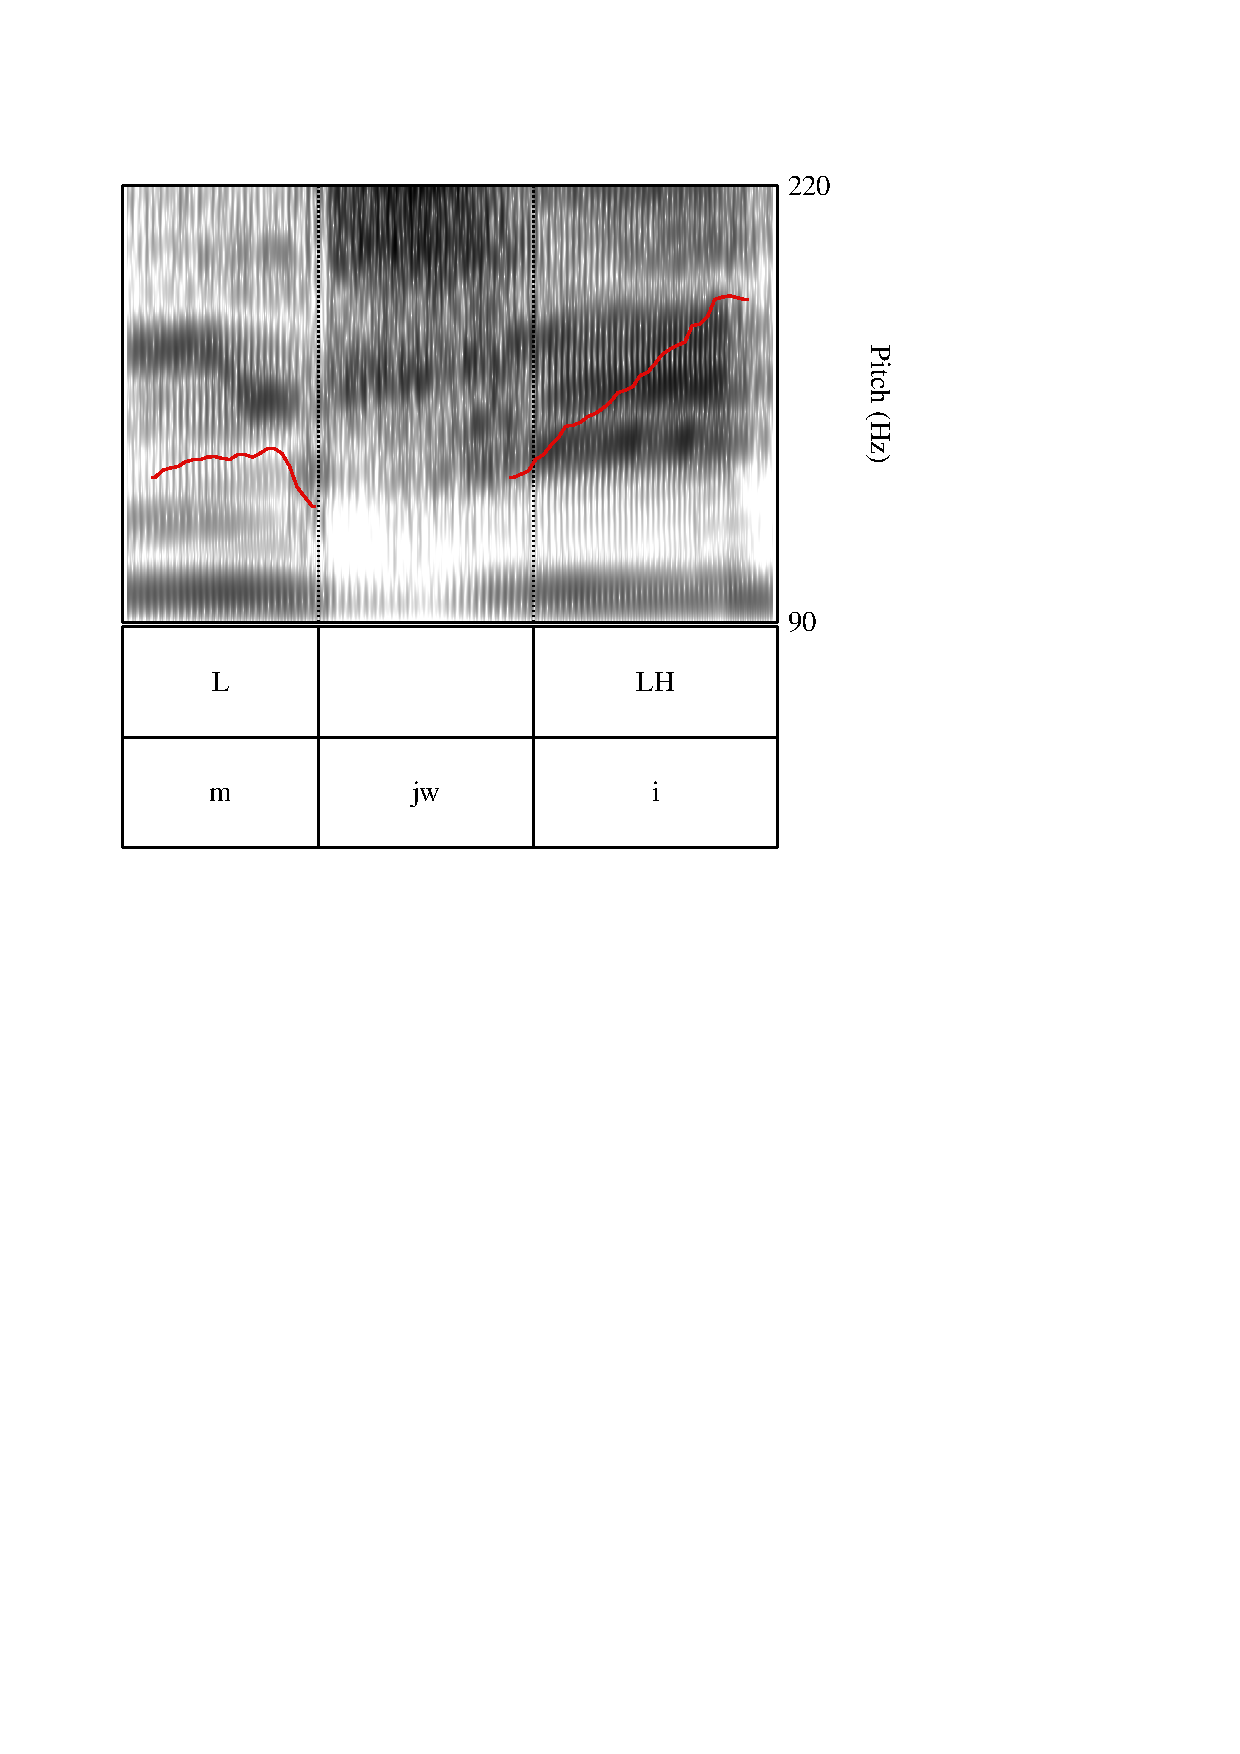
\includegraphics[width=8.5cm]{figures/fig1_mjwi.pdf}
\label{fig:riseV}
\end{figure}

\begin{figure}[p]
\caption{LH tone on syllable with coda /p/ -- /ŋkǎp/ [ŋkàp\'ə] `money'  (spoken in isolation)}
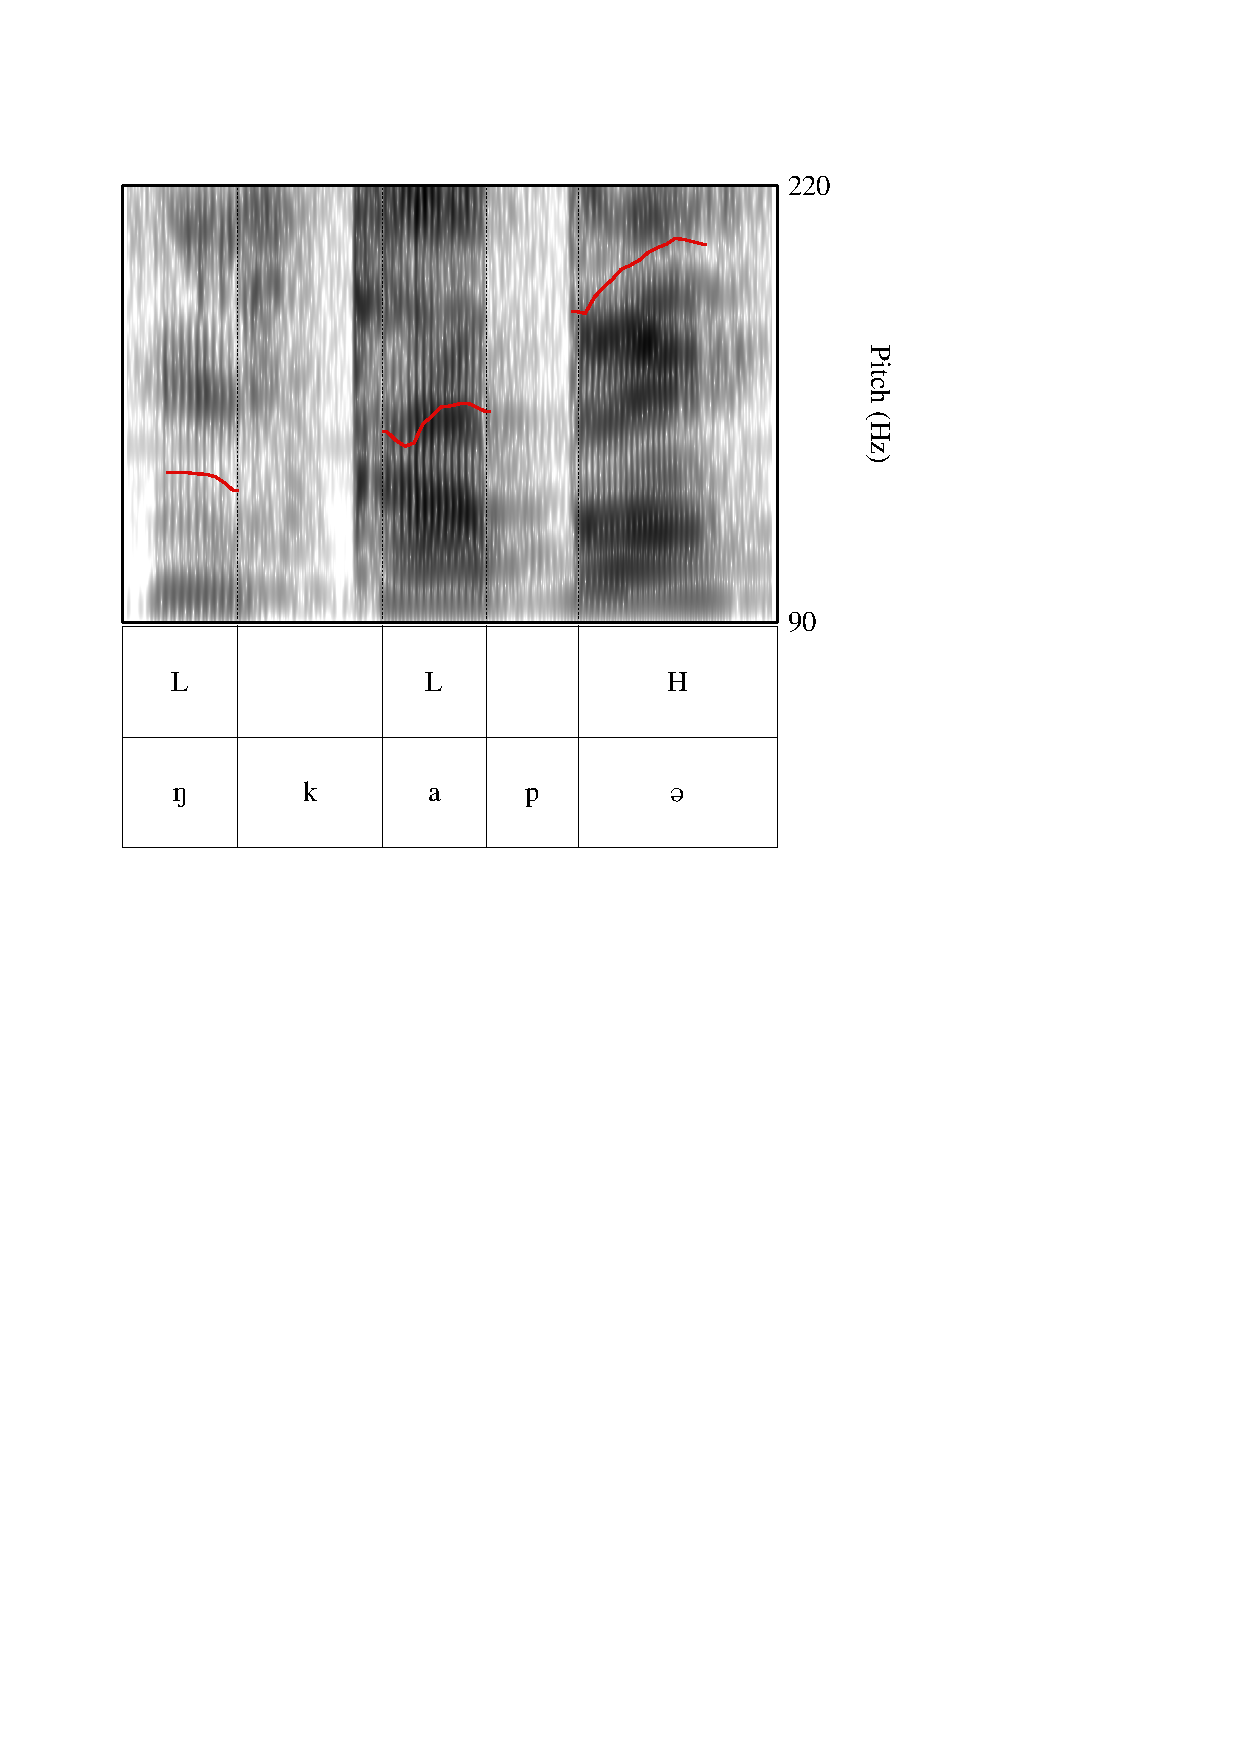
\includegraphics[width=8.5cm]{figures/fig2_nkape.pdf}
\label{fig:riseP}
\end{figure}

\begin{figure}[p]
\caption{L°{} tone on syllable with coda /p/ -- /bàp°/ `animal'  (spoken in isolation)}
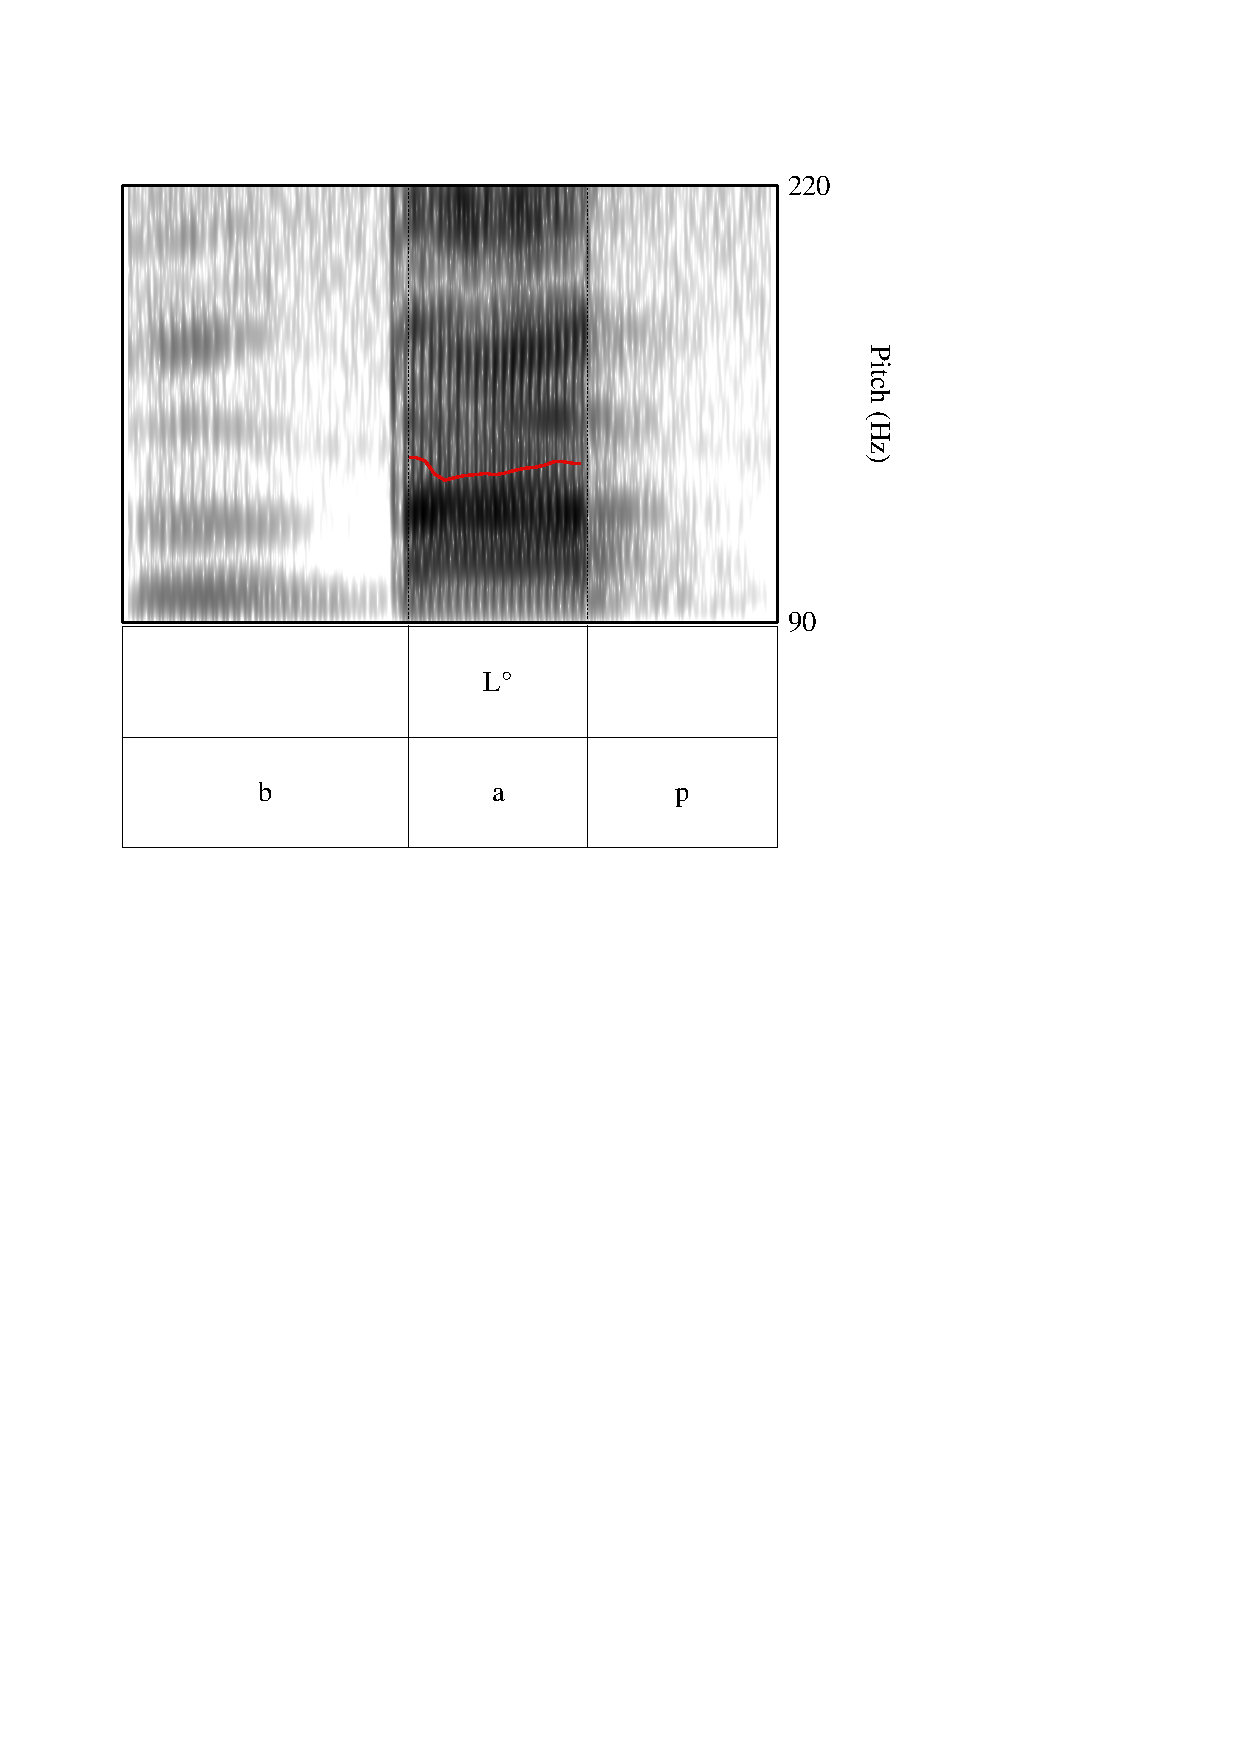
\includegraphics[width=8.5cm]{figures/fig3_bap.pdf}
\label{fig:levelP}
\end{figure}

\begin{figure}[p]
\caption{LH tone with sonorant coda -- /msǎŋ/ [msà\'{ŋ}] `birds'   (spoken in isolation)}
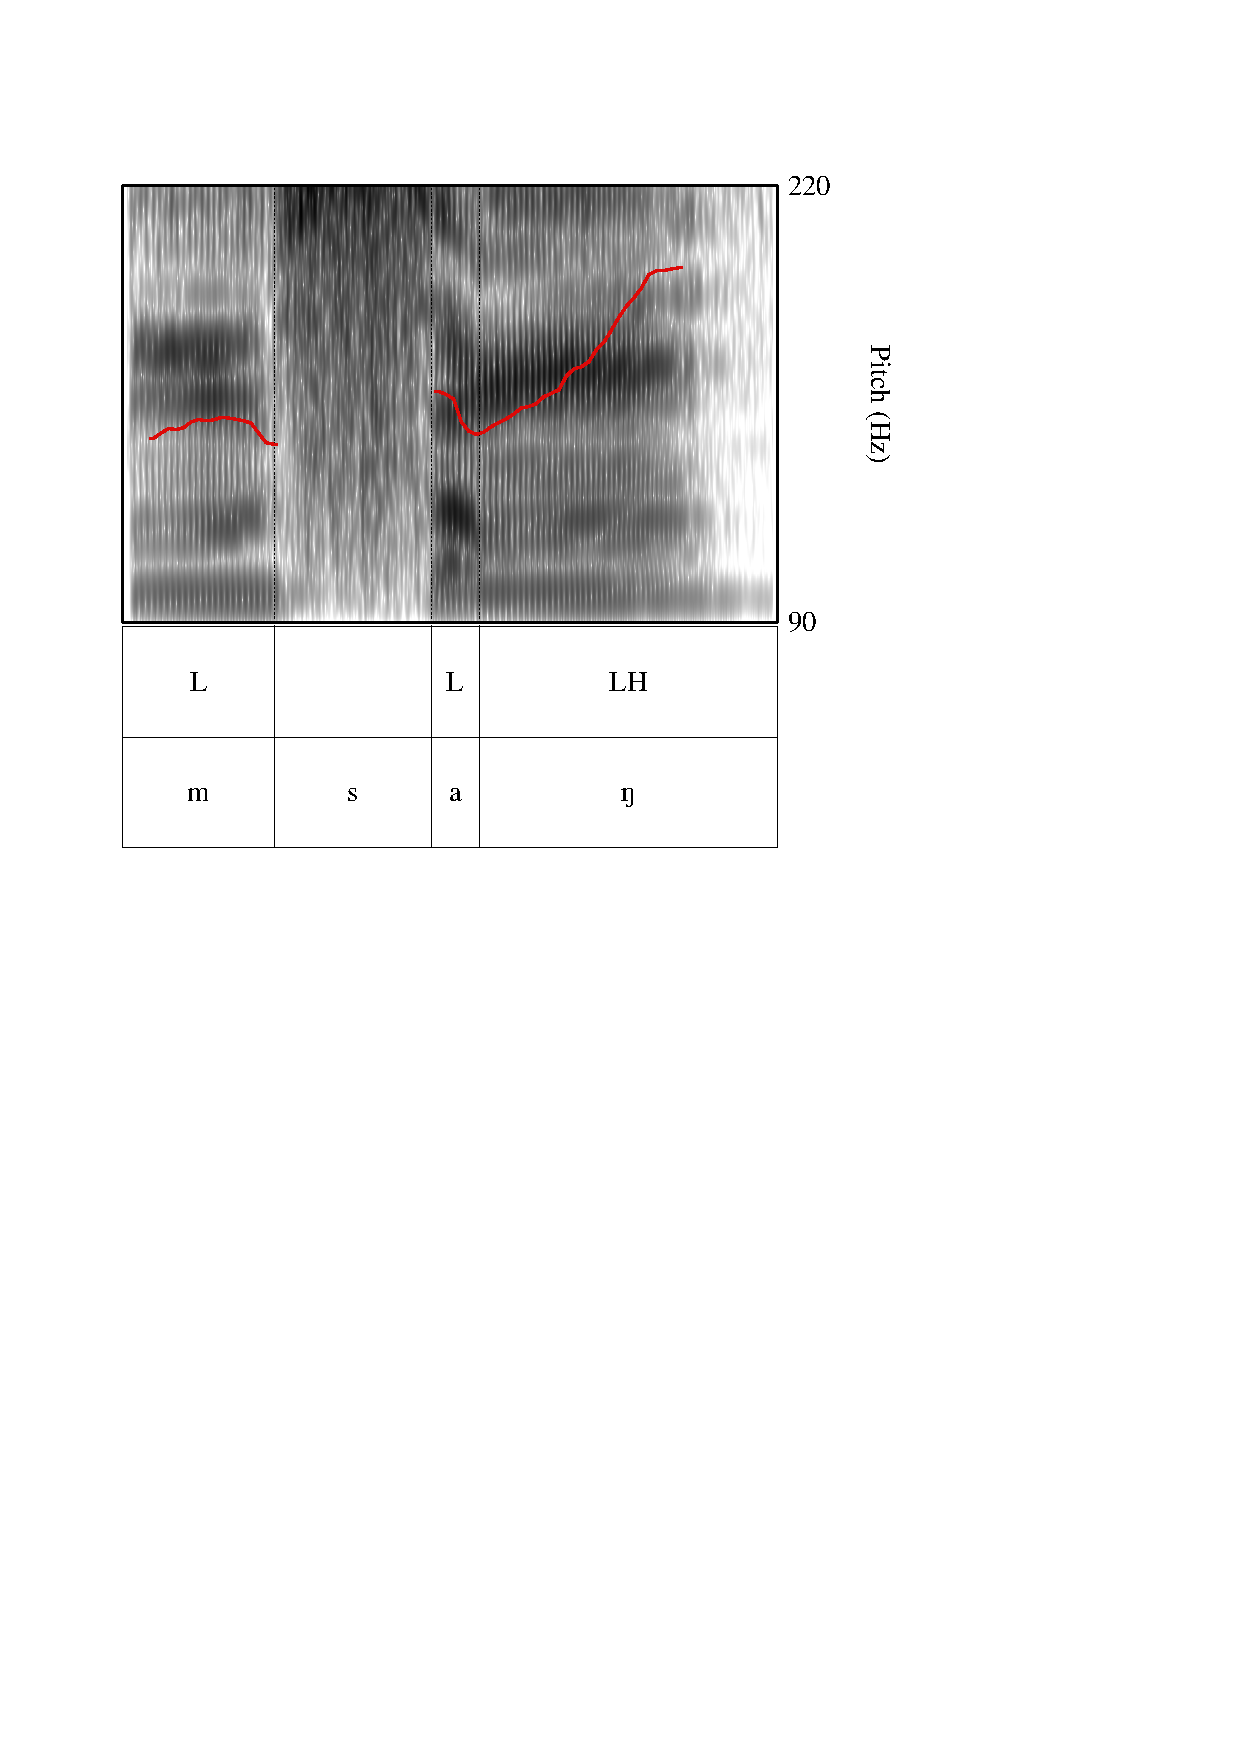
\includegraphics[width=8.5cm]{figures/fig4_msan.pdf}
\label{fig:riseN}
\end{figure}



Compare this to \figref{fig:levelP} which shows a level low tone (L°) on a syllable closed by the obstruent /p/.
Unlike \figref{fig:riseP}, here the /p/ is unreleased and no vowel follows it.
    % Parallel facts hold in the recordings involving coda /k/ and /ʔ/, not shown.
Moreover, unlike the coda obstruents, the coda nasals /m ŋ/ never show variants with an epenthetic vowel. 
A spectrogram confirms the lack of a final vowel in such LH contexts, shown in \figref{fig:riseN}.
It is clear  that the rising portion of the pitch is realized on [ŋ] itself.
These patterns show that the sonorant codas behave similarly  to open syllables in permitting a rising tone realization without recourse to epenthesis.


\subsection{Against a deletion alternative}

We now defend our analysis that this is indeed epenthesis, as opposed to an alternative hypothesis which would involve the  deletion of an underlying final vowel, i.e.  /\textsc{cvc}/ → [\textsc{cvc}ə], rather than  /\textsc{cvc}ə/ → [\textsc{cvc}].

The first argument involves  general root phonotactics.
As stated, the vast majority of roots in the language are monosyllabic (e.g. CV/CVC shapes). 
The major exception to this generalization are exactly those [\textsc{c\`{v}c}\'ə] forms detailed above.
If we treat these  as underlyingly /\textsc{c\v{v}c}/ which only become disyllabic later in the derivation,  this unifies the possible shape of roots.

Multisyllabic words which are not attributable to this epenthetic operation are nearly always decomposable into multiple morphemes. 
These include compounds of some type (e.g. \textit{n\`ɔm-g\"{w}\`{i}} `panther', more literally `animal-panther') or derived forms with a derivational affix (e.g. suffixes /-nyə/ and /-tə/ or the prefix /k\`ə-/).
Examples of the latter are given in (\ref{ex:suffix}). 
    % We return to such suffixes  in \sectref{sec:alter}.
Disyllabic sequences with final [ə] are in fact quite common in morphologically complex words, demonstrating that there is no general phonological constraint against final [ə] in Ghomala'.

\begin{exe}
	\ex Disyllabic stems as multi-morphemic (\citealt[91--92]{nissim1981}) \label{ex:suffix}
	    \begin{xlist}
		\ex 
		    k\`{u}ŋ-ny\`ə\\
		    love-\textsc{recip}\\
		    `love each other'
		\ex 
		    pà-t\`ə\\
		    carry.on.back-with.care\\
		    `carry carefully' (e.g. of a baby)
		 \ex 
		   k\`ə-l\'{o}ʔ \\
		   \textsc{depr}-? \\
		   `badly put together'
	    \end{xlist}
\end{exe}


Any remaining forms which cannot be decomposed into multiple morphemes constitute a marginal percentage of the lexicon, e.g. /b\`{i}y\'ɛ/ `peanut', /g\`əf\`{α}/ `corn', /k\'əpák/ `lizard', among others.
To this we can add loanwords from English and French found in \citet{eichholzer2010}, e.g. /b\`əl\`əŋ/ from English `blanket' or /bàt\^{o}/ `boat' from French \textit{bateau}.

The second argument for an analysis as epenthesis over one as deletion involves a restriction on the distribution of vowel quality.
Recall the vowel inventory /i, e, ɛ, ʉ, ə, α, a, u, o, ɔ/ of Ghomala'
presented in \tabref{tab:chart} (where α is IPA [ɐ]).
Of these, not all are permitted in closed syllables.
Before coda /p/ and /k/, only the low vowels /ɔ/ and /a/ are allowed (a few loanwords escape this generalization, e.g. /h\^ɛp/ `help' -- \citealt[21]{eichholzer2010}).
The data shown from \tabref{tab:pkcoda} above are representative of this restriction.

From a diachronic perspective, it is clear  that multiple vowel categories have merged in these closed syllable contexts.
Comparing Ghomala’ data to Proto-Eas\-tern Grassfields (Proto-EG)  reconstructions \citep{elias1984}, we see widespread neutralization before coda obstruents, such as before Proto-EG *b and *p codas shown in \tabref{tab:hist}.
Such data show that each of these distinct vowels in Proto-EG corresponds to a Ghomala' form with /ɔ/.

\begin{table}
\caption{Historical merger of vowel qualities before obstruent codas}
\label{tab:hist}
\begin{tabularx}{\textwidth}{lllllll}
\lsptoprule
    \multicolumn{3}{l}{Proto-EG \citep{elias1984}}
        % \footnote{The tone marks above the consonants in these proto-forms are reconstructed floating tones. We repeat the transcription as found in the source.}}
    && \multicolumn{2}{l}{Ghomala'} & Source\\
\midrule
    *-g\'{\c{u}}b\'&*chicken&(p. 52) &>&g\v{ɔ}p$\sim$g\`ɔp\'ə&`hen'&\citep[18]{eichholzer2010} \\
    *-k\'{i}b\' &*fingernail&(p. 90) &>&ŋk\`ɔp\'ə&`nail'&\citep[198]{nissim1981} \\
    *-b\'{o}p- &*fear&(p. 90) &>&pw\'ɔk&`afraid'& \citep[43]{nissim1972} \\
    *-b\'{e}b\`& *he-goat&(p. 59)&>& p\v{ɔ}p$\sim$p\`ɔp\'ə&`goat'& \citep[45]{eichholzer2010}\\
\lspbottomrule
\end{tabularx}
\end{table}


Importantly, this constraint holds both for [\textsc{cvk}] forms with a surface obstruent coda (e.g. [bàp°] `animal'), as well as  [\textsc{cvk}ə] forms with a surface [ə] (e.g. [gàp\'ə] `antelope').
    % showing counterbleeding opacity.
If the latter forms were underlyingly /\textsc{cvc}ə/ then we would have expected a wider range of vowels to be permitted, since the environment for the first vowel would not be a closed syllable on the surface.
In short, we would expect non-existent native roots such as /b\`{u}p\'ə/ and /g\`ɛk\'ə/.
Treating all such forms as underlying /\textsc{cvc}/ succinctly accounts for why such forms do not exist.
 
\subsection{Morpho-phonological alternations}\label{sec:alter}
This subsection details further support for our analysis as epenthesis, involving morpho-phonological alternations between surface forms with and without a final [ə].
These data demonstrate that tone-driven epenthesis is an active part of Ghomala' grammar.

Let us first consider data from derivation which show the parity between monosyllables and disyllables with final [ə] in the realization of LH tone.
In one type of deverbal nominalization, the lexical tone of the root is overwritten with LH tone, shown in \tabref{tab:deriv}. (Note that verb roots have only a H vs. L distinction -- see \sectref{sec:verbs} below).
With open syllables (row a) or syllables with coda sonorants (b), the pattern surfaces with a rising tone on a monosyllable without complication. 
In contrast, the LH pattern induces an epenthetic [ə] in syllables with coda obstruents (c), mirroring the distribution of underived roots in the lexicon. 

\begin{table}
\caption{[ə] alternations in V → N derivation (\citealt[288--289]{nissim1981})}
\label{tab:deriv}
 \begin{tabularx}{.8\textwidth}{lXllXl}
  \lsptoprule
a. & tʉ\`ɔ & `be strong' & → & tʉ\v{ɔ} & `iron' \\
 & s\'{u} & `(to) weed' & → & s\v{u} & `hoe' \\
b. & t\`{u}\ng & `dig inside' & → & nt\v{u}\ng & `throat' \\
 & t\'ɔm & `push' & → & t\v{ɔ}m & `fruit' \\
c. & ts\`{ʉ}ʔ & `twist' & → & dz\`{ʉ}ʔ\'{ʉ} & `liana (vine)' \\
 & f\'ɔk & `blow (cold)' & → & f\`ɔk\'ə & `cold' \\
  \lspbottomrule
 \end{tabularx}
\end{table}


Next, consider [ə] alternations in noun phrases, specifically in the associative construction.
To understand these data, first let us establish the relevant parts of this construction. 
Associative constructions are used to express possession and compounding, and involve two nouns where the first noun is the head and the second noun is the modifier.
We exemplify it in \tabref{tab:assoc}, involving various H- and L-toned nouns in N$_1$ position and the noun /bàp°/ `animal'
in the modifier position N$_2$.

\begin{table}
\caption{Class-dependent grammatical tone \citep[249--250]{nissim1981}}
\label{tab:assoc}
 \begin{tabularx}{\textwidth}{lXllllll}
  \lsptoprule
&Class&N$_1$&&N$_2$&&Output&Meaning\\
    \midrule
a. &\textsc{cl}1 & /m\'{u} &  Ⓛ  & bàp°/ & → & {[}m\^{u} bàp°{]} & `the child of the animal' \\
 && /g\`{i} &  Ⓛ  & bàp°/ & → & {[}g\`{i} bàp°{]} & `the voice of the animal' \\
b. &\textsc{cl}3 & /th\'ə &  Ⓗ  & bàp°/ & → & {[}th\'ə bàp°{]} & `the head of the animal' \\
 && /kw\`ə &  Ⓗ  & bàp°/ & → & {[}kw\`ə ꜜbàp°{]} & `the foot of the animal' \\
  \lspbottomrule
 \end{tabularx}
\end{table}

Notice that there are two classes  indicated here, class 1 (\textsc{cl1}, in row a) and class 3 (\textsc{cl3}, in b).
As is typical for related Bantu/Bantoid languages, Ghomala' has an elaborate noun class system which is reflected morphologically in the shape of morphemes that are in agreement with the head noun. 
In the associative construction,  noun class is reflected by distinct grammatical tones.
Class 1  nouns  condition a floating low grammatical tone (Ⓛ)
which links the two nouns (following \citealt{yip2002}, floating tones unassociated in the input are circled). 
In contrast, other classes (e.g. class 3) condition a floating high tone (Ⓗ).
These grammatical tones result in various tonal changes, e.g. in row a /m\'{u}/ becomes falling [m\^{u}], while in row b the second low tone becomes a downstepped low tone.
    % \footnote{In light of this downstep pattern, it may be more accurate to analyze the associative marker as a floating register feature ⓗ
    % rather than a floating tone Ⓗ.
    % This anticipates our discussion of tonal features in \sectref{sec:features} below,  so we shall not expand on this point here.
    % An analysis of this grammatical marker as ⓗ or Ⓗ
    % is not critical to our overall argument and we keep Ⓗ 
    % for the sake of simplicity.}


\citet{nissim1981} provides extensive paradigms of associative constructions. 
We schematize the relevant tonal patterns of these paradigms in Tables \ref{tab:cl1assoc} and \ref{tab:non1assoc}.
The underlying tones of the first noun (the head noun, N$_1$) are listed in the first column, and the underlying tones of the second noun (the modifier, N$_2$) are listed in the top row. 
\tabref{tab:cl1assoc} shows the tone paradigm for associative constructions involving a class 1 head noun (e.g. /m\'{u}/ `child' from \tabref{tab:assoc}).
Such environments condition the floating  Ⓛ  grammatical tone between  N$_1$ and  N$_2$.
Here, the tone of N$_2$ remains intact while the tone of   N$_1$  is altered.
In contrast, \tabref{tab:non1assoc} summarizes those constructions involving a class 3 head noun (e.g. /th\'ə/ `head').
These condition the floating Ⓗ  grammatical tone  between  N$_1$ and  N$_2$.
Here, it is the tones of N$_2$ that are modified, while those of N$_1$ remaining largely unmodified.

% \begin{samepage}
\begin{table}
\caption{Associative tone paradigm with \textsc{cl1} noun in N$_1$, conditioning floating Ⓛ}
\label{tab:cl1assoc}
 \begin{tabularx}{.9\textwidth}{X lr lr lr lr lr}
  \lsptoprule
N$_1$ / N$_2$  & \multicolumn{2}{c}{H} &  \multicolumn{2}{c}{ꜜH} & \multicolumn{2}{c}{L°}  &\multicolumn{2}{c}{L}  & \multicolumn{2}{c}{\textbf{LH}} \\
\midrule
H &   {[}HL & H{]} & {[}HL & H{]} & {[}HL & L°{]} & {[}HL & L{]} & \textbf{{[}HL} & \textbf{{LH}{]} }\\
L° &   {[}HL & H{]} & {[}HL & H{]} & {[}HL & L°{]} & {[}HL & L{]} & \textbf{{[}HL }&\textbf{ {LH}{]}} \\
L &   {[}L & H{]} & {[}L & H{]} & {[}L & L°{]} & {[}L & L{]} & \textbf{{[}L }&\textbf{ {LH}{]}} \\
LH &   {[}HL & H{]} & {[}HL & H{]} & {[}HL & L°{]} & {[}HL & L{]} & \textbf{{[}HL }& \textbf{{LH}{]}} \\
  \lspbottomrule
 \end{tabularx}
\end{table}
 
\begin{table}
\caption{Associative tone paradigm with \textsc{cl3} noun in N$_1$,  conditioning floating Ⓗ}
\label{tab:non1assoc}
 \begin{tabularx}{.9\textwidth}{X lr lr lr lr lr}
  \lsptoprule
N$_1$ / N$_2$  & \multicolumn{2}{c}{H} &  \multicolumn{2}{c}{ꜜH} & \multicolumn{2}{c}{L°}  &\multicolumn{2}{c}{L}  & \multicolumn{2}{c}{\textbf{LH}} \\
 \midrule
H &   {[}H & H{]} & {[}H & ꜜH{]} & {[}H & L°{]} & {[}H & L{]} & \textbf{{[}H} & \textbf{ꜜH{]}} \\
L°   & {[}L & H{]} & {[}L & H{]} & {[}L & ꜜL°{]} & {[}L & ꜜL{]} & \textbf{{[}L }& \textbf{H{]}} \\
L &   {[}L & H{]} & {[}L & H{]} & {[}L & ꜜL°{]} & {[}L & ꜜL{]} & \textbf{{[}L} & \textbf{H{]}} \\
LH &   {[}LH & H{]} & {[}LH & ꜜH{]} & {[}LH & L°{]} & {[}LH & L{]} & \textbf{{[}LH }& \textbf{ꜜH{]}} \\
  \lspbottomrule
 \end{tabularx}
\end{table}
% \end{samepage}

For our examination of tone-driven epenthesis, the relevant portions of both these tables are the rightmost columns (in bold).
For nouns in N$_2$ position with an underlying LH pattern, there are two surface realizations depending on the noun class of N$_1$.
If a class 1 noun is in N$_1$ position  (\tabref{tab:cl1assoc}), N$_2$ surfaces with a rising tone.
In contrast, if the noun of N$_1$ is class 3 (\tabref{tab:non1assoc}), N$_2$ surfaces with a downstepped high tone.\footnote{Notice in \tabref{tab:non1assoc} that the high tone of N$_2$ is not downstepped after a low tone. There is no contrast between [H] and [ꜜH] in this environment.}

This [LH]$\sim$[ꜜH] alternation surfaces as a purely tonal phenomenon in open syllables and in syllables with coda sonorants, e.g. /bvʉ̌/
[bvʉ̌]
$\sim$
[ꜜbvʉ́]
`dog' in (\ref{ex:dog}).

\begin{exe}
	\ex {[}LH{]}$\sim${[}ꜜH{]} morpho-phonological alternation in N$_2$  \label{ex:dog}
	    \begin{xlist}
		\ex 
		    /m\'{u} Ⓛ   bv\v{ʉ}/ → [m\^{u} bv\v{ʉ}] `the child of the dog' \citep[264]{nissim1981}
        \ex 
		    /th\'ə   Ⓗ  bv\v{ʉ}/ → [th\'ə ꜜbv\'{ʉ}] `the head of the dog' \citep[153]{nissim1981}
	    \end{xlist}
\end{exe}

\noindent Importantly, when there is a coda obstruent, N$_2$ nouns show the expected co-variation between tonal pattern and the presence of a final epenthetic vowel.
Consider the noun /gɔ̌p/ `hen' 
which in isolation is pronounced [gɔ̀pə́].
\citet[157--158, 250--252]{nissim1981} provides the paradigms  in \tabref{tab:hen} which show that in the surface [LH] context this surfaces as [gɔ̀pə́]
with a final vowel (a), but in the surface [ꜜH]  context it surfaces as
[ꜜgɔ́p]
without the final schwa (b).

\begin{table}
\caption{Co-variation between tone pattern and the presence of a final {[}ə{] in morpho-phonological alternations} \citep[157--158, 250--252]{nissim1981}
}
\label{tab:hen}
 \begin{tabularx}{\textwidth}{lXllllrl}
  \lsptoprule
a. & /mú &   Ⓛ   & gɔ̌p/ & → & {[}mû & gɔ̀pə́{]} & `the child of the hen' \\
 & /kòʔ° &   Ⓛ   & gɔ̌p/ & → & {[}kôʔ & gɔ̀pə́{]} & `the rooster of the hen' \\
 & /gì &   Ⓛ   & gɔ̌p/ & → & {[}gì & gɔ̀pə́{]} & `the voice of the hen' \\
 & /dyə̌ &   Ⓛ   & gɔ̌p/ & → & {[}dyə̂ & gɔ̀pə́{]} & `the house of the hen' \\
b. & /thə́ &  Ⓗ  & gɔ̌p/ & → & {[}thə́ & ꜜgɔ́p{]} & `the head of the hen' \\
 & /mkòʔ° &  Ⓗ  & gɔ̌p/ & → & {[}mkòʔ & gɔ́p{]} & `the roosters of the hen' \\
 & /kwə̀ & Ⓗ  & gɔ̌p/ & → & {[}kwə̀ & gɔ́p{]} & `the foot of the hen' \\
 & /tǎŋ &  Ⓗ  & gɔ̌p/ & → & {[}tǎŋ & ꜜgɔ́p{]} & `the ear of the hen' \\
 \lspbottomrule
 \end{tabularx}
\end{table}


Recordings made by Ghomala' language advocates and teachers confirm this distribution in morpho-phonological alternations. 
Consider the following recording  publicly available on YouTube, titled \textit{Animaux en ghomala}.\footnote{This is available at \url{https://www.youtube.com/watch?v=M5S1Pmw4ND8}, by speaker Kamdem Wambo.} 
The speaker speaks in the Baham variety, which is part of the central Ghomala' dialect very closely related and geographically proximate to Bandjoun.
The recording contains individual names of common domesticated and wild animals within the Ghomala' environs, as well as several basic nouns and noun phrases in isolation. 

% Several of these words involve a rising tone and/or an obstruent coda.
In this recording, open syllables or syllables with sonorant codas with rising tones surface as expected, e.g. [ts\v{ə}] `elephant' (at 9\textquotesingle 33$"$ in the video) and [bàpd\v{ə}m] `rat' (3\textquotesingle 15$"$).
There are also 28 instances of a root with an obstruent coda, and all 28 comply with the expected patterns of epenthesis. 
Representative examples are in \tabref{tab:baham}, which provides a sample of  words  with coda consonants of all tone patterns.
Each word in this table is accompanied by its corresponding entry in the Ghomala' dictionary \citep{eichholzer2010}.
If the obstruent coda occurs with H, HL, L°, or L tone, then the form ends with a consonant.
However,  if it occurs with a LH tone (e.g. [s\^{ʉ} p\`ɔb\'ə] `castrated goat'), then the word ends in an epenthetic vowel (row e).

\begin{table}
\caption{Corroborating evidence for tone-driven vowel epenthesis from the \textit{Animaux en ghomala} video (Baham variety of Central dialect)}
\label{tab:baham}
 \begin{tabularx}{\textwidth}{llllXl}
  \lsptoprule
&Tone & \multicolumn{2}{l}{Example}   &Location&Cf.  \citet{eichholzer2010}\\
    \midrule
a.&H& [n\'ɔk] &`snake'& (13\textquotesingle 31$"$)&[n\'ɔk] `snake'\\
b.&HL &[dz\^ɔp]& `hedgehog'& (16\textquotesingle 20$"$)&[dz\^ɔp]  `hedgehog'\\
c.&L°{} &[\ng gàp°{}] &`antelope'&(11\textquotesingle12$"$)&[gàp°] `antelope'\\
d.&L &[kwàk] &`jigger flea' &(32\textquotesingle 02$"$)&[kwàk] `jigger' \\
% &&&&&&(French \textit{chique})\\
e.&LH& [s\^{ʉ} p\`ɔb\'ə] & `castrated goat'& (6\textquotesingle 51$"$)&[s\'{ʉ}] `castrate' \&  \\
&&&&&[p\v{ɔ{}}p]$\sim$[p\`ɔp\'ə] `he-goat'\\
 \lspbottomrule
 \end{tabularx}
\end{table}


\figref{fig:baham1} shows that the root /g\v{ɔ}p/ `chicken' is realized in this video  as [g\'ɔp] with a high tone and no final epenthesis when spoken in isolation.\footnote{Faint aspiration can be detected in the recording, on this and many other obstruent-final tokens.
Due to noise in the recording, however, it is more difficult to clearly see on the spectrogram. 
The indeterminacy of aspiration is notated as `(h)' in \figref{fig:baham1}.}
Although this pronunciation of a rising tone as high in isolation is different from the data from the Bandjoun variety (cf. Tables \ref{tab:obscoda} and \ref{tab:hist}), it still supports our main thesis since there remains strict co-variation between tone and epenthesis. 
This is confirmed by \figref{fig:baham2} of the noun phrase [m\^{ʉ} g\`ɔb\'ə] `chick' (lit. `baby chicken').
Here, the final noun is realized as [LH], with the low portion hosted on the lexical vowel and the high portion on an epenthetic vowel [ə], as expected.

\begin{figure}
\caption{H tone without epenthesis -- [g\'ɔp] `chicken' spoken in isolation (24\textquotesingle 28$"$)}
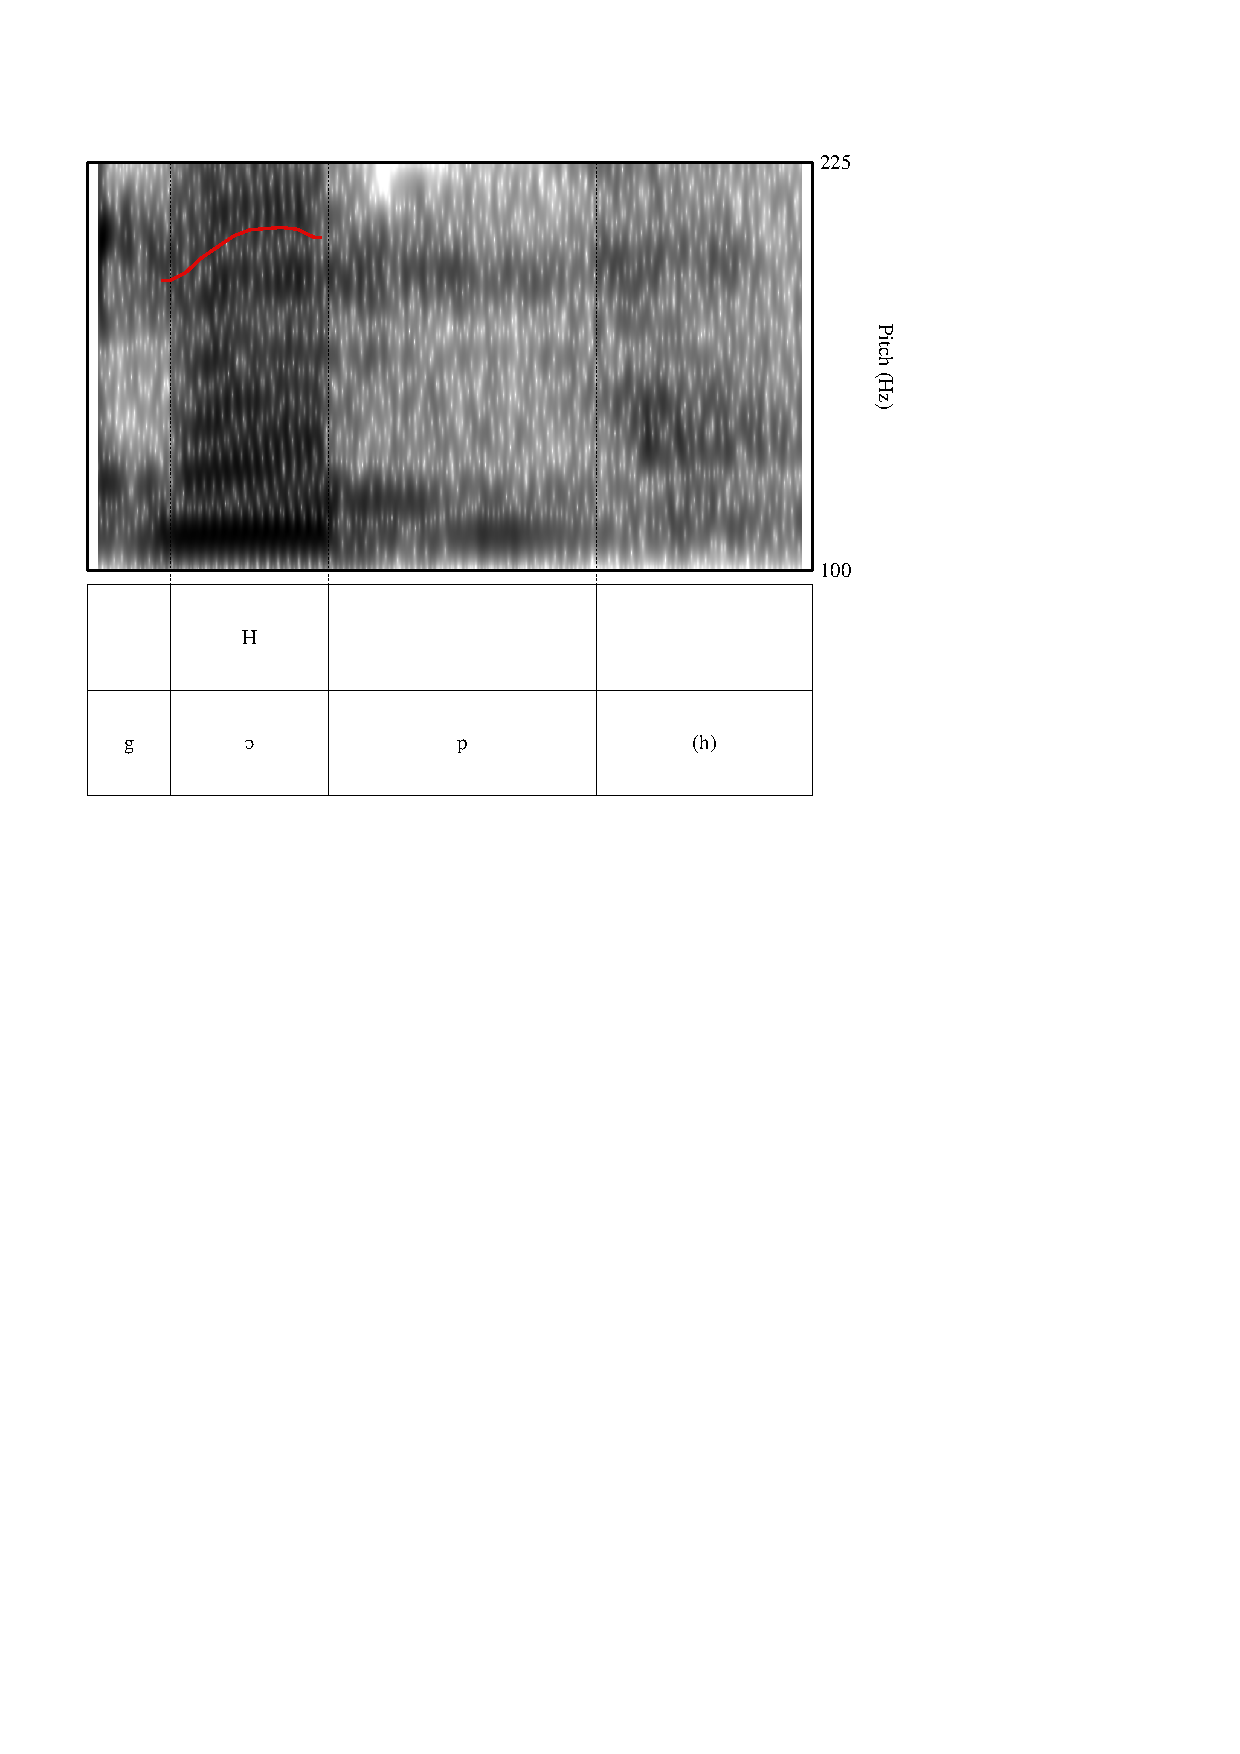
\includegraphics[width=9.5cm]{figures/fig5_AEG_gop.pdf}
\label{fig:baham1}
\end{figure}

\begin{figure}
\caption{LH tone \textit{with} epenthesis --[m\^{ʉ} g\`ɔb\'ə] `chick'  (25\textquotesingle 10$"$)}
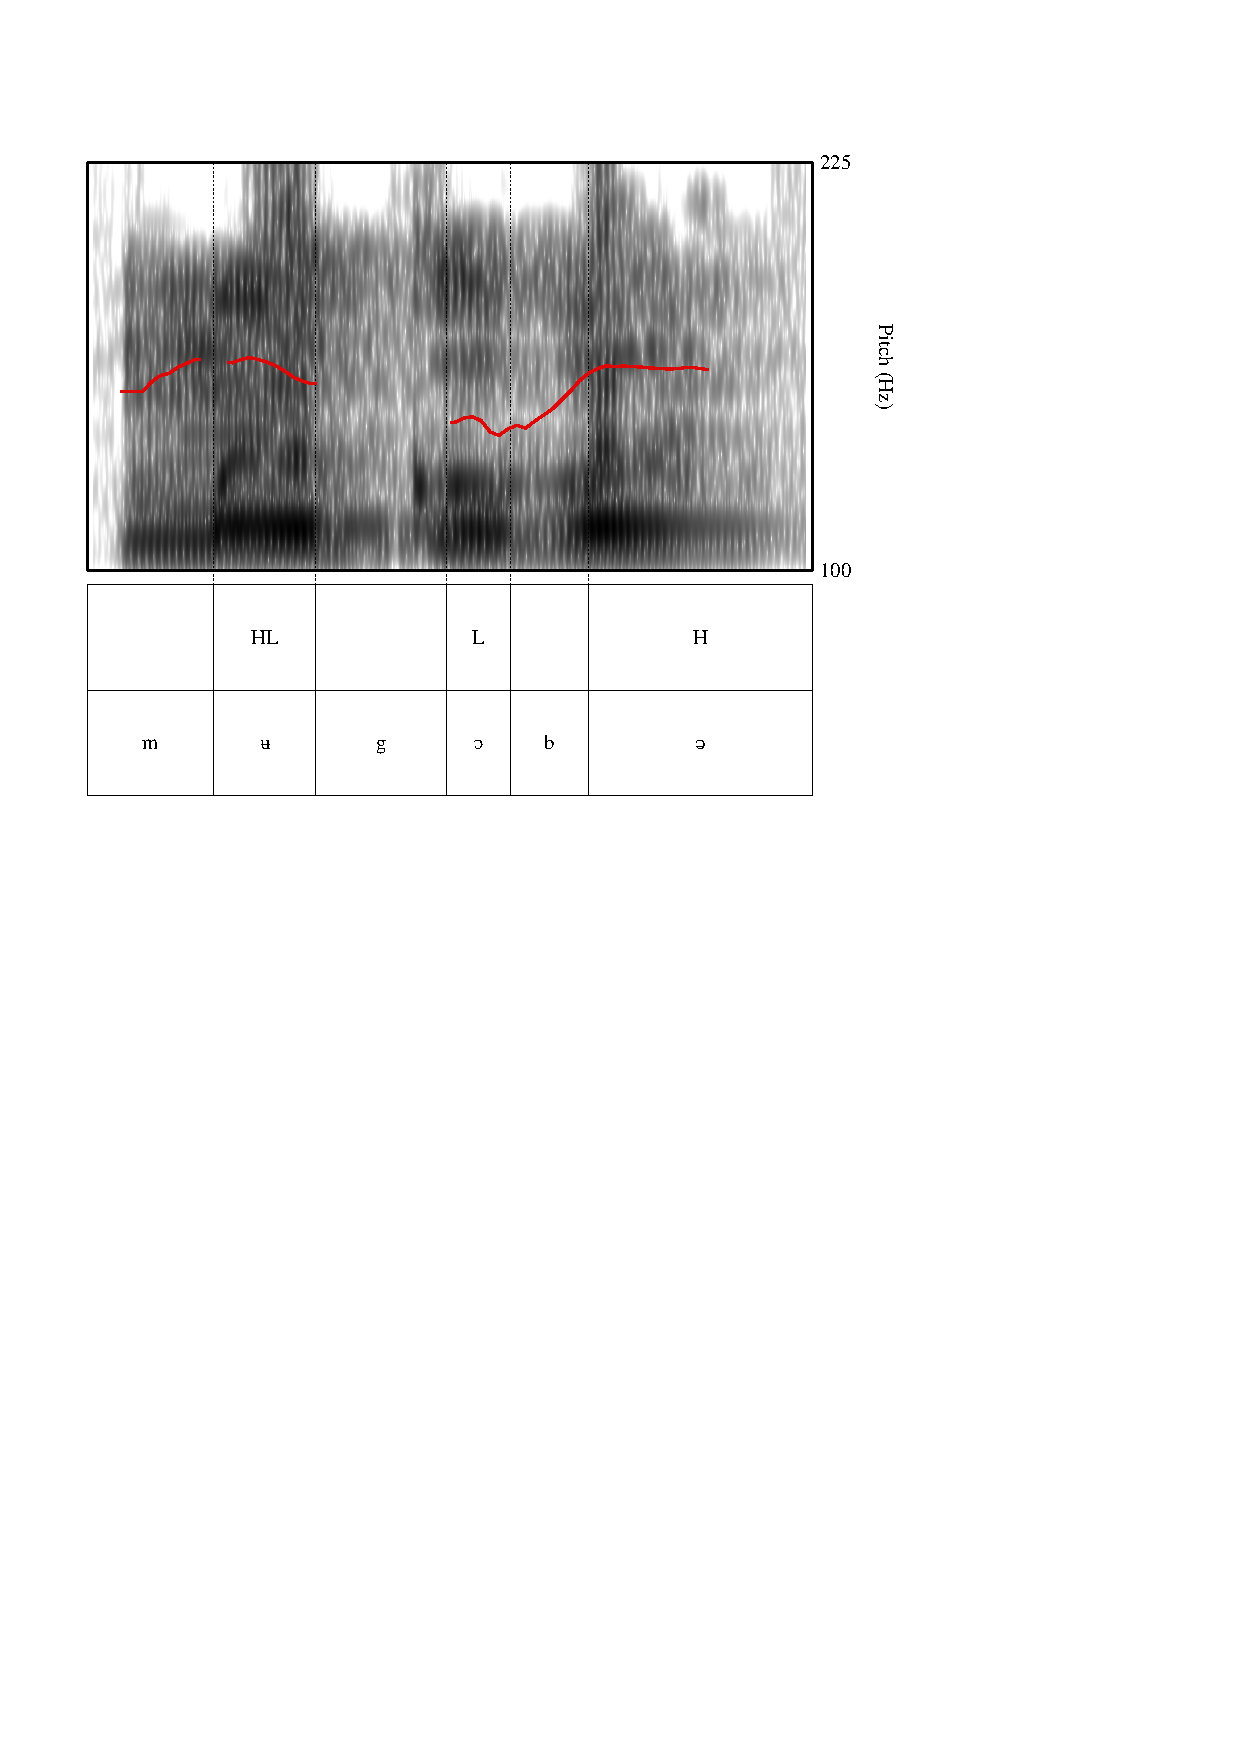
\includegraphics[width=9.5cm]{figures/fig6_AEG_mU_gObE.pdf}
\label{fig:baham2}
\end{figure}

\subsection{Indeterminate data from verb inflection}\label{sec:verbs}

To wrap up our discussion of tone-driven epenthesis in Ghomala', we  provide a final note on a set of indeterminate data from verb inflection. 
Unlike nouns, Ghomala' verb roots have  only a basic underlying H vs. L distinction  (\citealt[79]{nissim1972}, \citealt[78]{mba1997}), a property the language shares with other Bamileke languages \citep[62]{elias1984}. 
Parts of the verbal system confirm the observations made for the nominal domain, e.g. for L-toned roots the imperative is expressed with LH tone realized as a rising tone on roots like [pàá]
`carry on the back!' but with an epenthetic [ə] on roots like [càpə́]
`insult!' \citep[80]{nissim1972}.
However, other parts of the system complicate our generalizations. 

Consider the data in (\ref{ex:bessala}) from \citet{bessala2017}  involving the lexically low-toned verb /ʒw\`ɔp/ `dance' (in bold in the example).
Here, too, there is an alternation between an obstruent coda and a final [ə].
Note that this source transcribes the level low tone (i.e. L°) as a mid tone, which we repeat.\footnote{There are other orthogonal changes as well, such as changes to the initial consonant of the verb. These are not relevant to our discussion.}

\begin{exe}
	\ex \label{ex:bessala}
        \begin{xlist}
            \ex \gll 		    bə́jə̄ pō \textbf{ʒwɔ̄p} áá, bə̄ gâ nə̄ŋ \\
            \textsc{cond} you \textbf{sing} \textsc{def} \textsc{cond} I dance\\
             \glt `If you sing then I will dance.' \citep[153]{bessala2017}
            \ex \gll 	tâmō bə̄ wə̄ \textbf{dʒwɔ́pə́} \\
            Tamo \textsc{cop}  \textsc{prog}  \textbf{sing}\\
            \glt `Tamo is singing.' \citep[151]{bessala2017}
        \end{xlist}
\end{exe}

\noindent While the form in (a) without epenthesis complies with our  analysis, the form in (b) is unexpected, since it shows a final [ə] not co-occurring with a LH tone. We cannot attribute the presence of [ə] here to the avoidance of a rising tone on a syllable closed by an obstruent. 

The presence of this inflectional `final vowel' has been noticed already in the literature on Ghomala'  (\citealt{bessala2017}, \citealt[100]{kamdem2020}),
but at this point its  function and distribution are not yet established. 
To complicate things further, variability is common even within the same inflectional context.
For example, one context where this final vowel appears is with lexically low-toned roots in the infinitive, e.g. /càp/ `insult' surfaces as [šápə̀°]
`to insult' \citep[77]{nissim1972}.
While  Nissim more or less consistently transcribes final vowels in such infinitival contexts, in  sources such as \citet{mba1997} (of the same Bandjoun dialect) there is no indication of such vowels in equivalent contexts.
This is exemplified in \tabref{tab:infinitive}.
No final vowel appears in either source with roots of the H tone class (row a), but the sources differ as to whether another vowel is added with roots of the L tone class (b). (Notice as well that Mba  indicates infinitives with an initial prefix \textit{n\'ə}-, while Nissim often has initial consonant changes in infinitive context.)

\begin{table}
\caption{Variation for infinitive forms across sources}
\label{tab:infinitive}
 \begin{tabularx}{\textwidth}{lllllXl}
  \lsptoprule
 & \multicolumn{2}{l}{Tone class}&   & \textsc{inf} \citep{nissim1972} & \textsc{inf} \citep{mba1997} & Meaning \\
 \midrule
a.  &   H   &   fíʔ                 & &     [fìʔ°]       & [nə́-fîʔ] & `to descend' \\
    &       &   s\'ɛ   & &     [s\`ɛ°]     & [n\'ə-s\^ɛ]  & `to count' \\
b. &L& fìʔ &  & [fíʔì°] & [nə́-fìʔ] & `to water' \\
 && vɔ̀k &  & [bvɔ́χə̀°] & [nə́-vɔ̀k] & `to live (on)'\\
    &       &   pà   & &     [báà°]     & [n\'ə-pà]  & `to carry on  back' \\
\lspbottomrule
\end{tabularx}
\end{table}

In total, while tonal-driven epenthesis can be firmly established for nouns, the situation with verbs requires further data and analysis. 

 
\section{Tone-driven epenthesis in a typological perspective}\label{sec:discussion}
In the previous section, we have shown that Ghomala' disprefers a rising tone on a syllable closed by an obstruent.
We can call this the *[\textsc{c\v{v}k}] constraint. 
To avoid such a structure, a final vowel is epenthesized which hosts  the high tone portion of the contour (i.e. a word /g\v{ɔ}p/ becomes [g\`ɔp\'ə] `hen').
Evidence came from root phonotactics as well as  morpho-phonological alternations, showing that this is an active part of the Ghomala' phonological grammar. 

In this section, we situate the Ghomala' *[\textsc{c\v{v}k}] constraint and tone-driven epenthesis in a cross-linguistic perspective, with comparison to similar types of patterns in various languages.
We divide this section into three parts.
In \sectref{sec:constraints}, we discus how both rising tones and syllables closed by an obstruent are marked structures with respect to tone-segment interaction.
In this perspective, a *[\textsc{c\v{v}k}] constraint is exactly the type of constraint that is expected to emerge.
\sectref{sec:repairs} shows, however, that tone-driven epenthesis as a repair is  vanishingly rare if not unprecedented.
Finally, \sectref{sec:intonation} discusses an important parallel to tone-driven epenthesis, namely intonation-driven epenthesis whereby a vowel is inserted to host part of an intonational tune.
Although intonation-driven epenthesis has been purported more often than tone-driven epenthesis, it too is rare cross-linguistically.

\subsection{The commonality of constraints on rising contours}\label{sec:constraints}
The	*[\textsc{c\v{v}k}] constraint of Ghomala' is a particular manifestation of two cross-linguistic markedness patterns: one pertaining to rising contours, and one pertaining to the ability of syllables closed by an obstruent to host tone.
Let us begin with the former. 

In a large-scale survey of contour tones, \citet{zhang2013} finds that if a language only allows one type of contour (falling or rising), languages which only allow surface falling tones (\textit{n}=37) far exceed those which only allow surface rising tones (\textit{n}=3).
Furthermore, Zhang finds in numerous languages that rising tones have a more limited distribution than falling tones, such as with respect to syllable type or position within the word.
In Mende \il{Mende}
[\href{https://glottolog.org/resource/languoid/id/mend1266}{\texttt{men}}], for example, a HL falling contour can occur on the final syllable of a disyllabic word while a LH rising contour cannot.
Such cross-linguistic findings warrant the phonological markedness scale in (\ref{ex:markedness})  \citep{yip2002,hyman2007}, where level tones are less marked than falling tones, which are less marked than rising tones. 

\begin{exe}
	\ex  Markedness scale of tones (from less marked to more marked):\\  \label{ex:markedness}
	\{H,L\} > F > R
\end{exe}

Let us now consider the second markedness type. 
A large literature now exists which evaluates which syllable types are better hosts for tone and appear with a larger range of tone types, and which are worse. 
Surveys of contour tones (e.g. \cite{gordon2001,zhang2013}) find a cross-linguistic  implicational hierarchy.
If a syllable that ends in a sonorant/resonant (what we shall abbreviate as `CVN') can carry a contour, then a long vowel (`CVV') can carry a contour of ``equal or greater tonal complexity'' \citep[49]{zhang2013}. 
Moreover, if a syllable that ends in an obstruent (which we shall abbreviate as `CVK') carries a contour, then CVN and CVV syllables can as well. 
Zhang shows that this implicational hierarchy is clearly seen in many Chinese languages. 
In the Changzhou variety of Wu Chinese   \il{Wu Chinese}
[\href{https://glottolog.org/resource/languoid/id/wuch1236}{\texttt{wuu}}], for example,  
five types of tone may appear on CVV/CVN syllables -- 55, 13, 523, 24, and 45 (where 1 is the lowest and 5 the highest) -- while only two tones may appear on CVK syllables -- 23 and 5 \citep{wang1988changzhou}.
This implicational hierarchy can be captured in a markedness scale parallel to the one posited above in (\ref{ex:markedness}).
This is shown in (\ref{ex:syllmarkedness}).\footnote{Note that we specifically do not place short syllables (i.e. CV) in this scale. While \citet[428]{gordon2001} finds  that ``if a language allows contour tones on CV, it also tolerates them on [CVK], [CVN], and CVV'', there are exceptions to this such as Ghomala' itself.}

\begin{exe}
	\ex  Markedness scale of a syllable's ability to host a tone contour:\\  \label{ex:syllmarkedness}
	CVV > CVN > CVK
\end{exe}


\citet[11]{hyman2007} connects these two scales, stating that ``in principle, the more complex (`marked') a tone is, the more likely it is to...be restricted to a hospitable TBU (e.g. a long, prominent, sonorous TBU)''. 
One exemplification of these two scales interacting comes from  Standard Thai
[\href{https://glottolog.org/resource/languoid/id/thai1261}{\texttt{tha}}]     \il{Thai}
\citep{gandour1975representation},
discussed by \citet{yip2002}.
Gandour follows a common approach to tone-segment interactions in Asian languages, dividing syllables into `smooth' syllables (e.g. ending in a nasal, glide, or vowel, i.e. CVN) versus checked syllables (e.g. ending in a stop such as [p t k ʔ], i.e. CVK).
There are five tones in Thai -- high, mid, low, falling, and rising -- but not all tones are allowed on both syllable types, summarized in \tabref{tab:thai}.\footnote{Marginal words which \citet[172]{gandour1975representation} mentions include \textit{k\textsuperscript{h}l\^{a}k} `be crowded' with a falling tone on a CVK syllable and \textit{káát} `gas' (a loanword) with high tone on a CVVK syllable. Importantly, Gandour is explicit that ``mid and rising tones never occur on a checked syllable''.}
This table shows that rising but not falling contours show a categorical ban in certain syllabic environments. 
These syllabic environments are exactly the ones we would expect from the markedness scale in (\ref{ex:syllmarkedness}).
To this, we can add the Ghomala' constraint *[\textsc{c\v{v}k}] as one further instantiation of the interaction of these two scales. 


\begin{table}
\caption{Thai tone type by syllable type
    (Y=possible,
    (*)=marginal,
    *=impossible) \citep{gandour1975representation}}
\label{tab:thai}
 \begin{tabularx}{\textwidth}{llll CCCCC}
  \lsptoprule
 &  & Syllable &  & High & Mid & Low & Falling & Rising \\
 \midrule
a. &  & CVV &  & Y & Y & Y & Y & Y \\
b. &  & CVN &  & Y & Y & Y & Y & Y \\
c. &  & CVVN &  & Y & Y & Y & Y & Y \\
d. &  & CVK &  & Y & \cellcolor[HTML]{9B9B9B}* & Y & \cellcolor[HTML]{C0C0C0}(*) & \cellcolor[HTML]{9B9B9B}* \\
e. &  & CVVK &  & \cellcolor[HTML]{C0C0C0}(*) & \cellcolor[HTML]{9B9B9B}* & Y & Y & \cellcolor[HTML]{9B9B9B}* \\
\lspbottomrule
\end{tabularx}
\end{table}



While the above discussion is based around phonological typology, accumulated research in phonetics corroborates the particular markedness of [\textsc{c\v{v}k}] sequences.
It is well-known that of contour tones, rising pitch takes longer to execute than falling pitch, and consequently a rising tone has greater duration on average (e.g. \citealt{sundberg1973,zhang2013}).
Moreover, the main phonetic correlate of tone is  fundamental frequency (i.e. \textit{f}$_0$), and rich harmonic structures are crucial to the perception of \textit{f}$_0$.
Because sonorous segments such as vowels and sonorants possess richer harmonic structures than obstruents, pitch targets are better perceived on them.
It therefore follows that syllables with obstruents would make for worse tone-bearing units generally, which would be compounded by the complexity of the tone.
Taking these two aspects together, [\textsc{cvk}] structures may not provide enough sonorous material to adequately realize the rising tone within its allotted duration.
 

\subsection{The rarity of tone-driven epenthesis as a repair}\label{sec:repairs}

In response to  such phonetically motivated pressures, phonological systems respond in various ways.
The simplest case are  those languages which unequivocally prohibit [\textsc{c\v{v}k}]-type structures, which we saw in Thai (\tabref{tab:thai}).
In many languages, however, syllables closed by obstruents (or other inadequate hosts for contours)  are `repaired' in some way.
One common repair is to lengthen the vowel (which may or may not neutralize a phonological distinction between short vs. long vowels).
For example, \citet{zhang2013} cites lengthening in Mitla Zapotec [\href{https://glottolog.org/resource/languoid/id/mitl1236}{\texttt{zaw}}] \il{Mitla Zapotec}
for syllables with rising contours, which does not apply to  falling contours \citep{briggs1961}.
Another common repair involves the compression, simplification, or flattening of the rising contour (see Zhang for examples).
These two repairs are two sides of the same coin: 
there is a discrepancy between the amount of duration the syllable has versus the amount that the tone requires, and either the vowel lengthens or the tone compresses to accommodate. 

In contrast, tone-driven epenthesis as a repair to  a *[\textsc{c\v{v}k}] constraint (or a similar  constraint)  is exceedingly rare if not unprecedented. 
No such repair is mentioned in either of the large-scale typological surveys mentioned above \citep{gordon2001,zhang2013}.
Nor does it appear in reference works on tone (e.g.
\citealt{pike1948},
\citealt{fromkin1978},
\citealt{yip2002},
\citealt{wee2019}, 
\textit{inter alia}),
or on epenthesis (e.g.
\citealt{broselow_predicting_1982},
\citealt{ito_prosodic_1989},
\citealt{blumenfeld2006},
\citealt{de2006markedness},
\citealt{hall_cross-linguistic_2006},
\citealt{hall2011},
\textit{inter alia}).
In fact, works which posit a maximally restrictive theory of epenthesis assume tone-driven epenthesis to be impossible/unattested \citep{blumenfeld2006,gleim2019}.
Blumenfeld concludes that epenthesis is ``used exclusively as a response to pressures of syllable structure, sonority sequencing, syllable contact, and word minimality'' (p. 5), but that ``tone conditions cannot affect string structure'' and therefore tone ``cannot force epenthesis/syncope'' (p. 41).

It is, therefore,  quite remarkable that an epenthetic vowel in Ghomala' appears in order to host part of a pitch contour, rather than being solely due to segmental or syllabic markedness.
Other than Ghomala', we are aware of only four potential cases of tone-driven epenthesis: in Wamey, Kejom, Barain, and Arapaho. 
Of these, only Wamey looks as convincing as the Ghomala' case.

Wamey \il{Wamey}
[\href{https://glottolog.org/resource/languoid/id/wame1240}{\texttt{cou}}] (also called Konyagi/Coniagui)
is a language of Guinea and Senegal, traditionally placed in the ``Atlantic'' group of the Niger-Congo phylum (and only distantly related to Ghomala').
In a recent paper, \citet{rollemerrill2022} provide a number of arguments parallel to those developed for Ghomala', building on earlier description and insights found in \citet{santos1996}. 
Like in Ghomala', in Wamey rising tones on closed syllables trigger epenthesis.
This is evidenced by restrictions on the shape of roots. 
Wamey has a basic H vs. L tone contrast, and HL and LH contours are common.
As summarized in \tabref{tab:wamey}, in isolation monosyllabic CVC-shaped roots may bear H, L, or HL tones, but no CVC root appears with a LH tone.
At the same time, bisyllabic CVCə-shaped roots are not permitted with H, L, or HL patterns, but only appear with the LH tone.

\begin{table}
\caption{Complementary distribution in Wamey of bisyllabic CVCə vs monosyllabic CVC surface root shapes, based on  tone \citep{santos1996}}
\label{tab:wamey}
 \begin{tabularx}{\textwidth}{lllXlll}
  \lsptoprule
&Tone&	\multicolumn{2}{l}{Roots with surface  [CVCə]}& &\multicolumn{2}{l}{Roots with surface  [CVC]} \\
 \midrule
a.&H&*\textsc{cv́c}ə́&&	& [cǽw̃] &	`urinating'\\
b.&L&*\textsc{cv̀c}ə̀&&	& [cæ̀w̃] &	`hiding'\\
c.&HL&*\textsc{cv́c}ə̀&&	& [cæ̂w̃] &	`domestic animal'\\
d.&LH&[nkæ̀w̃ə́]&	`dance'&& *\textsc{cv̌c}	&\\
\lspbottomrule
\end{tabularx}
\end{table}

This complementary distribution is naturally captured by a unified underlying representation /CVC/ for all four root types, plus tone-driven [ə] epenthesis to avoid a rising tone on a closed syllable.
As in Ghomala' the overwhelming majority of roots are monosyllabic, and those CVCV structures which cannot be attributed to the epenthesis operation are either morphologically complex or  loanwords.

We cannot attribute  epenthesis here to segmental phonotactics, which would prohibit certain consonants in coda position. 
For any closed syllable bearing  a rising LH tone, epenthesis is triggered. 
In Wamey, this applies with all coda consonants, not just by an obstruent as in Ghomala'.
All consonants are otherwise allowed in coda position, shown in  (\ref{ex:implosive}).
(Note that the prefixes are noun class markers, not relevant to our discussion).

\begin{exe}
	\ex \label{ex:implosive}
	    \begin{xlist}
        	\ex H   [ì-gwǽlǽɓ] ‘to talk a lot’	
        	\ex L  [ì-còɓ] ‘to stick on’
		    \ex HL    [æ̀-kæ̂ɓ] ‘rubber vine’
		    \ex LH  [æ̀-kə̀ɓə́] ‘a species  of owl’ (\textit{Otus leucotis})	
	    \end{xlist}
\end{exe}


\newpage
Moreover, Wamey also demonstrates morpho-phonological alternations supporting the equivalency of coda-final and [ə]-final forms.
For example, the suffix /-k/ (roughly equivalent to third person singular perfective) is one of several suffixes which show alternations of the type [-k]$\sim$[-kə́].
The data in (\ref{ex:ksuffix}) are representative for the distribution of the two variants: the [-k] form appears if the preceding vowel is high-toned (a),
while the [-kə́]
variant appears if the preceding vowel is low-toned (b).
Such alternations are accounted for if we posit that the final schwa in (b) is inserted in order to avoid a rising tone on a syllable closed by /-k/ (see \citealt{rollemerrill2022} for extensive argumentation).

\begin{exe}
	\ex Tone-driven alternations in Wamey \citep[43]{santos1996} \label{ex:ksuffix}
	    \begin{xlist}
	        \ex After [H]: 	\textit{ì-cǽs}	‘to suffer’  → 	\textit{cǽsə́-k} 	‘he suffers’
	        \ex After [L]: 		\textit{ì-tòk}	‘to eat’   → \textit{tókə̀-kə́}	‘he ate' (cf. *tókə̌-k)
 	    \end{xlist}
\end{exe}


While Wamey is a strong candidate for tone-driven epenthesis, the three other cases are much weaker.
The first is another Grassfields language of Cameroon closely related to Ghomala', namely 
Kejom \il{Kejom}
[\href{https://glottolog.org/resource/languoid/id/baba1266}{\texttt{bbk}}]
(also called Babanki).
The relevant data involve various verb inflection paradigms, found in \citet{akumbu_segmental_2020}.
For example, the authors analyze the imperative (specifically the non-indicative singular imperative) as involving  a floating 
 Ⓗ
tone which appears after the verb.
Representative imperative data are in (\ref{ex:kejom1}), with high-toned and low-toned roots.
If Ⓗ
appears with a high-toned root (e.g. /lám/ `cook'), then no overt marking is observed.
However,  if it appears with a low-toned root (e.g. /k\`{u}m/ `touch'), 
then an overt inflectional suffix [-ə] appears.
Note that in this example, there is high tone spreading onto the object's noun class prefix /kə̀-/, resulting in a surface mid tone.

% \begin{samepage}
\begin{exe}
	\ex Non-indicative singular imperative in Kejom \citep[11]{akumbu_segmental_2020} \label{ex:kejom1}
	    \begin{xlist}
	        \ex 	H root:	/lám Ⓗ kə̀-báyn/	→	[\textbf{lám} kə̄-báyn]		‘Cook the fufu!’
	        \ex L root:		/kùm Ⓗ kə̀-báyn/	→	[\textbf{kùmə́} kə̄-báyn]	`Touch the fufu!'
 	    \end{xlist}
\end{exe}
% \end{samepage}

\noindent \citet[3]{akumbu_segmental_2020} specifically characterize this distribution as lexically low verb roots having ``acquired an epenthetic schwa to avoid the rising tone that would otherwise result from combining the root L with the H suffix tone of the imperative (*\textit{kǔm})''.
This would constitute tone-driven epenthesis. 

However, one aspect of Kejom which makes it distinct from Ghomala' and Wamey is that this epenthesis process is not regular across verbal paradigms.
For example, in the analogous context under negation, no epenthesis is found.
As \citet{akumbu_segmental_2020} make clear, the same imperative floating  Ⓗ 
must be present in (\ref{ex:kejom2}) as well,
since it conditions tonal changes on the object.

\begin{exe}
	\ex Non-indicative negative singular imperative  \citep[14]{akumbu_segmental_2020} \label{ex:kejom2}
	    \begin{xlist}
	        \ex 	/kə́ à lám Ⓗ kə̀-báyn/	→	[ká \textbf{ꜜlám} kə̄-báyn]		‘Don’t cook the fufu!’
	        \ex /kə́ à kùm Ⓗ kə̀-báyn/	→	[ká \textbf{kùm} kə̄-báyn]			‘Don’t cook the fufu!’
 	    \end{xlist}
\end{exe}
 
\noindent 
If tone-driven epenthesis were fully regular in Kejom, we would expect the unattested form *[kùmə́] 
in (b).

Another similar case which falls short of tone-driven epenthesis is found in Barain [\href{https://glottolog.org/resource/languoid/id/bare1279}{\texttt{bva}}] \il{Barain}
(Chadic: Chad -- \citealt{lovestrand_linguistic_2012}).
In Barain, tone alone cannot condition epenthesis but rather  makes otherwise variable segmentally-driven epenthesis obligatory.
\citet[21]{lovestrand_linguistic_2012} details the strict requirements on complex onsets and codas, showing that an epenthetic vowel is inserted to satisfy these requirements. 
In (\ref{ex:barain}), the vowel [i] is inserted to break up the heteromorphemic consonant cluster.

\begin{exe}
	\ex  Barain epenthesis \label{ex:barain} \citep[44]{lovestrand_linguistic_2012}\\
	/wīĺs-gà/ ‘boil-\textsc{do:3.m}’	 →
	[wīls\textbf{í}g{à}]
\end{exe}


Speakers differ as to whether they manifest epenthesis in such heteromorphemic contexts.
A coarse generalization is that younger speakers consistently insert epenthetic vowels in such cases while older speakers show more variation.
This is exemplified in \tabref{tab:barain} with two speakers, A (of the younger generation, who consistently shows epenthesis) and B (of the older generation, who is more variable).

Importantly, \citet[63]{lovestrand_linguistic_2012} states that even ``those speakers who allow the unlicensed cluster still prefer the epenthetic vowel in the case where not using the epenthetic vowel would create a word with fewer [tone-bearing units] than underlying tones''. 
One example involves the imperfective aspect realized as a floating Ⓜ tone 
(row b from \tabref{tab:barain}).
When such a floating tone is present,  epenthesis is required by all speakers, and its absence is questionable/ungrammatical.
In Barain, therefore, tone alone does not condition epenthesis per se, but rather increases the preference for it.\footnote{Two things should be noted in this table: a regular tonological rule changes  M to L before  L, and questionable forms are notated with a superscript $^?$ as compared to ungrammatical forms which are marked with an asterisk.}


\begin{table}
\caption{Barain epenthesis co-driven by both segmental structure and tone \citep{lovestrand_linguistic_2012}}
\label{tab:barain}
 \begin{tabularx}{\textwidth}{llXll}
   \lsptoprule
     & Morphemes & Gloss & Speaker    A & Speaker B (Older gen.) \\
    \midrule
a. & /s\'{e}\'{e}b-t\`{i}/ & fish-\textsc{do:3.f} &   {[}s\'{e}\'{e}b\textbf{\'{i}}t\`{i}{]} &  {[}s\'{e}\'{e}b\textbf{\'{i}}t\`{i}{]}  $\sim$  {[}s\'{e}pt\`{i}{]} \\
 & /\={e}p-gà/ & punish-\textsc{do:3.m} &   {[}\`{e}p\textbf{\`{i}}gà{]} &   {[}\`{e}p\textbf{\`{i}}gà{]}  $\sim$    {[}\`{e}pgà{]}\\
 & /pás̄-n\`{u}/ & miss-\textsc{do:1.s} &   {[}pás\textbf{\`{u}}n\`{u}{]} & {[}pás\textbf{\`{u}}n\`{u}{]} $\sim$  {[}pásn\`{u}{]} \\
b. & /d\'{o}p-Ⓜ-gà/
 & find-\textsc{ipfv}-\textsc{do:3.m} &   {[}d\'{o}p\textbf{\`{i}}gà{]} & {[}d\'{o}p\textbf{\`{i}}gà{]} (cf. $^?${[}d\'{o}pgà{]})\\
 & /s\'{e}\'{e}b-Ⓜ-gà/
& fish-\textsc{ipfv}-\textsc{do:3.m} &   {[}s\'{e}\'{e}b\textbf{\`{i}}gà{]} & {[}s\'{e}\'{e}b\textbf{\`{i}}gà{]}   (cf. $^?${[}s\'{e}bgà{]}, \\
&&&&{ } { } { } { } { } { } { } { } { } { } { } *{[}s\'{e}\`{e}bgà{]}) \\
\lspbottomrule
\end{tabularx}
\end{table}


Finally, a similar case comes from Arapaho [\href{https://glottolog.org/resource/languoid/id/arap1274}{\texttt{arp}}] \il{Arapaho}
(Algonquian: USA -- \citealt{Cowell2008}).
This superficially resembles tone-driven epenthesis, but \citet{gleim2019} argues it is better understood as `tone-driven retention'.
Here, vowels that are otherwise expected to delete according to the regular phonology are retained if and only if they bear tone.
Several such cases of tone-driven retention have previously been identified in 
\citet[279--280]{roettger2019}, e.g. in
Cheyenne \il{Cheyenne}
[\href{https://glottolog.org/resource/languoid/id/chey1247}{\texttt{chy}}],
Acoma \il{Acoma}
[\href{https://glottolog.org/resource/languoid/id/west2632}{\texttt{kjq}}],
Konso \il{Konso}
[\href{https://glottolog.org/resource/languoid/id/kons1243}{\texttt{kxc}}],
Japanese \il{Japanese}
[\href{https://glottolog.org/resource/languoid/id/nucl1643}{\texttt{jpn}}],
and the Shanghainese variety of Wu Chinese
[\href{https://glottolog.org/resource/languoid/id/wuch1236}{\texttt{wuu}}].
In general, our presentation of the Arapaho data here follows the argumentation developed in \citet{gleim2019}. 

In Arapaho, certain morphemes idiosyncratically co-occur with a floating high tone, shown in \tabref{tab:arapaho}.
In many contexts, this floating high  appears on an epenthetic vowel [i]/[u].
In row a, the epenthetic vowel and its surrounding consonants are in bold.
In contrast, if the morpheme does not sponsor a floating tone, then no surface epenthetic vowel occurs (row b).
Such data demonstrate a co-occurrence of floating tones and epenthetic vowels, which reasonably could be interpreted as tone-driven epenthesis.

\begin{table}
\caption{Arapaho epenthetic vowels and floating tones \citep{gleim2019}}
\label{tab:arapaho}
 \begin{tabularx}{\textwidth}{lXXl}
  \lsptoprule
a.&	/tʃew-Ⓗsee/		&		[tʃe\textbf{bís}ee]		&		‘to walk along’\\
&/oow-Ⓗsee/		&		[hoo\textbf{wús}ee]	&		‘to walk downward’\\
&/nééʔeeθ-Ⓗnihíí-noo/ &		[nééʔee\textbf{sín}ihíínoo]	&	‘that’s what I’m saying’\\
b.&	/étʃex-nówoʔ/		&		[hétʃe\textbf{sn}ówoʔ]		&	‘small fish’\\
&/nih-bebíiθ-tii-t/	&		[nihbebíi\textbf{st}iit]		&	‘s/he fixed it’\\
&/tʃew-kóóhu/			&	[tʃe\textbf{bk}óóhu]&			‘run along’\\
\lspbottomrule
\end{tabularx}
\end{table}

However,  \citet{gleim2019} argues that it is not epenthesis that is triggered by the floating tone here, but rather an epenthetic vowel is merely retained by the presence of tone which otherwise would have been deleted (building on original observations in \citealt[16]{Cowell2008}). 
The crucial evidence comes from a develarization process apparent, also seen in \tabref{tab:arapaho}:
velar segments /x/, /k/, \mbox{/w/} become [s], [tʃ], [b] before front vowels [i] and [e].
Crucially, develarization  takes place both before surface [i] (e.g. [tʃe\textbf{b}ísee]
in row a, where /w/→[b]),
as well as opaquely applying where no surface vowel appears (e.g. [hétʃe\textbf{s}nówoʔ] 
in row b, where /x/→[s]).

Gleim shows that the opacity can be accounted for straightforwardly if we assume  a `Duke-of-York derivation' \citep{pullum1976}, where an operation of vowel epenthesis applies first and uniformly,
followed by floating tone docking and develarization.
After these operations, an operation of high vowel deletion takes place, but only if the high vowel does not bear high tone (hence, tone-driven retention).
Because this deletion process can target an epenthetic vowel, the underlying form and the surface form look alike, characteristic of all Duke-of-York examples in the literature (i.e. of the type A → B → A). 

To summarize, 
in Kejom tone-driven "epenthesis" is not fully regular across the verb inflection paradigms, 
in Barain   tone alone cannot condition epenthesis but rather only makes otherwise variable segmentally-driven epenthesis obligatory,
and in Arapaho what resembles tone-driven epenthesis is actually tone-driven retention.
Ghomala' and Wamey, in turn, do not have  these shortcomings.
 
\subsection{A parallel: intonation-driven epenthesis}\label{sec:intonation}
A noteworthy  process comparable to tone-driven epenthesis exists in the intonation literature: intonation-driven epenthesis.
Here, a vowel is inserted to host part of an intonational tune (and not a lexical/grammatical tone per se).

Intonation-driven epenthesis can be situated within a larger discussion of ``text-tune" relationships in the intonation literature.
In cases where there is a mismatch between the segmental structure (the ``text") and the intonational melody (the ``tune"), normally it is the melody which accommodates (e.g. through truncation). 
A growing literature shows evidence for the opposite as well: segmental structure changing to accommodate the intonation 
\citep{roettger_tonal_2017,grice_word_2018,roettger2019}.

To illustrate, consider a recent study of Tunisian Arabic  \il{Tunisian Arabic}
[\href{https://glottolog.org/resource/languoid/id/tuni1259}{\texttt{aeb}}]
intonation \citep{hellmuth2022}.
Yes-no questions are commonly realized with a rise-fall intonational complex (i.e. L*+H H-L\%) at the right edge of an intonational phrase. 
When this intonational complex appears, it often co-occurs with an epenthetic vowel to which part of this complex docks.
An example of phrase-final [ə] epenthesis is in (\ref{ex:ta}).

\ea \label{ex:ta}
\gll 
nkemmil t\textsuperscript{ʕ}uːl → {} {} {} {} {} {} {} {[nkemmil t\textsuperscript{ʕ}uːləː]}\\
I-continue straight.ahead\\
\glt `Should I go straight ahead?' \citep{hellmuth2022}
\z
\il{Tunisian Arabic}

\noindent
Epenthesis only appears in the context of this complex rise-fall contour, and even then only  half the time. 
Importantly, it \emph{never} appears when there is only a simple rise or simple fall, even in the context of a yes/no question. 
Tunisian Arabic thus shows co-variation between a final vowel and a complex pitch event, suggestive of intonation-driven epenthesis.\footnote{Note, however, that \citet{hellmuth2022} deliberates over the final [ə] in examples like (\ref{ex:ta}) as to whether it is intonation-driven epenthesis or intonation-driven retention (analogous to Arapaho  in \tabref{tab:arapaho}).
She ultimately concludes that it is ``rather a ``question vowel" particle of some type'', analogous to similar interrogative clitics in the linguistic area. 
This speaks to the analytic indeterminacy of epenthesis, which is notoriously difficult \citep{morley_deletion_2015}.
Regardless, these Tunisian Arabic data suffice to illustrate intonation-driven epenthesis for our purposes.}





What unifies tone-driven and intonation-driven epenthesis is that both are attributable to a functional pressure to cultivate segmental environments best suited for realizing pitch targets.
Still, intonation-driven epenthesis is quite rare within the world's languages, though there are more purported cases than for tone-driven epenthesis.
See the above-mentioned sources for several other purported cases of intonation-driven epenthesis (especially \citealt{roettger2019}).

\section{Conclusion}\label{sec:conclusion}
This chapter focused on a little-known tonological rarity: tone-driven vowel epenthesis. 
We showed that in Ghomala', an epenthetic vowel is inserted to avoid a rising tone on a syllable closed by an obstruent, e.g. /g\v{ɔ}p/ → [g\`ɔp\'ə] `chicken', but never triggered in other tonal contexts.
We supported tone\hyp driven epenthesis with evidence from root phonotactics and morpho-phonological alternations which show that when a rising tone is modified the epenthetic vowel is lost (i.e. complete co-variation).
Finally, we situated these Ghomala' patterns within a larger cross-linguistic perspective. 
We demonstrated that the Ghomala' constraint against [\textsc{c\v{v}k}] structures has much typological and phonetic support, given the general markedness of rising contours, as well as the markedness of obstruent\hyp final syllables acting as tone-bearing units.
While the motivation for tone\hyp driven epenthesis is clear, we examined  all other purported cases of tone\hyp driven epenthesis and showed that nearly all of them fall short compared to Ghomala'.
We ended our study by comparing the Ghomala' patterns to a similar intonation-driven epenthesis, which, too, is  seldom reported for the world's intonational systems. 

There is one matter which has been conspicuously absent from our discussion thus far: if tone-driven epenthesis is so exceedingly rare, why?
Its existence in Ghomala' entails that we cannot deny it as a universal constraint, requiring a more nuanced explanation.
One possibility we would like to put forward involves functional load \citep{hockett1955manual,hockett1966quantification,wedel2013high,hall2019phonological}.
Cross-linguistically, lexical and functional meaning cued by tone can also be cued simultaneously by a co-occurring segmental component, and only more rarely cued by tone alone. 
Because of this, if tone is fully or partially deleted in some environment, the meaning can still be recovered in general.
In this way, the functional load of tone is quite low.
In many tonal languages, therefore, there is little reason to excessively maintain tone contrast if other markedness considerations come into play.
If there is enough segmental material to differentiate the morpheme from other paradigmatically-related morphemes (e.g. all nominal roots, or all tense/aspect suffixes), then adding more segmental material via epenthesis may be costlier than being faithful to the underlying tone pattern.

In short, because of the low functional load of tone, in most languages if the H portion of a hypothetical [\textsc{c\v{v}k}] sequence were  simply deleted, little information would be lost to correctly identifying the intended meaning.
At this point, such an  explanation  remains tentative, and a dedicated study is required before it can be evaluated further.

\section*{Abbreviations and glossing}
\begin{tabularx}{.45\textwidth}{lQ}
    {\'{\hphantom{a}}} (H) & high tone\\
    {ꜜ\'{\hphantom{a}}} (ꜜH) & downstepped high\\
     {\={\hphantom{a}}} (M) & mid tone\\
    {\`{\hphantom{a}}} (L) & low tone\\
    {\`{\hphantom{a}}°} (L°) & level low tone\\
    {\^{\hphantom{a}}} (F)  & falling tone\\
    {\v{\hphantom{a}}} (R)  & rising tone\\
    Ⓗ&floating high tone\\
    Ⓜ&floating high tone\\
    Ⓛ&floating low tone\\
    C&consonant\\
    V&vowel\\
    N&sonorant (in syllable)\\
    K&obstruent (in syllable)\\
    N$_1$&first noun in phrase\\
    N$_2$&second noun in phrase\\
\end{tabularx}
\begin{tabularx}{.45\textwidth}{lQ}
    \textsc{cl} & noun class\\
    \textsc{cond} & conditional\\
    \textsc{cop} & copular\\
    \textsc{def} & definite\\
    \textsc{depr} & depreciative\\
    \textsc{do} & direct object\\
    \textsc{f} & feminine\\
    {\textsc{h\_pst}} & hodiernal past\\
    \textsc{inf} & infinitive\\
    \textsc{infl} & inflection\\
    \textsc{ipfv} & imperfective\\
    \textsc{m} & masculine\\
    \textsc{prog} & progressive\\
    \textsc{recip} & reciprocal\\
    \textsc{s} & singular\\
    & \\
\end{tabularx}


\section*{Acknowledgements}
For  important feedback,
thanks go to 
Larry M. Hyman, 
Jack Merrill, 
Frank Kügler,
James Kirby,
Bob Ladd,
Joey Lovestrand, 
Ryan Gehrmann,
audiences at talks given at Goethe Universität Frankfurt and Ludwig Maximilians Universität München,
the anonymous reviewers, and
the editors of this book.
For technical support, thanks go to Sebastian Nordhoff at Language Science Press.

\printbibliography[heading=subbibliography,notkeyword=this]

\end{document}
